% Tento soubor nahraďte vlastním souborem s obsahem práce.
%=========================================================================
% Autoři: Michal Bidlo, Bohuslav Křena, Jaroslav Dytrych, Petr Veigend a Adam Herout 2019

\chapter{Úvod}

Tato práce se zabývá návrhem a tvorbou informačního systému pro firmu, zabývající se prodejem nátěrových hmot. Cílem práce je vytvořit přehledný firemní systém, ve kterém bude jednoduchá orientace a žádné zbytečné prvky, které by zastiňovaly nejdůležitější prvky systému, které budou uživatelé využívat nejčastěji. V rámci informačního systému by mělo být zákazníkům umožněno jednoduché vytvoření a následná správa jejich objednávek. Zaměstnanci firmy, kteří se systémem budou pracovat, budou mít přehled o všech objednávkách, které zákazníci vytvořili a budou moci jednoduše měnit stav, ve kterém se právě nachází a označovat provedenou práci. Zaměstnanci budou také mít přehled o všech objednávkách v rámci Google kalendáře. V rámci informačního systému budou k dispozici statistiky týkající se zejména prodeje produktů, ale i další. V informačím systému bude implementována také analýza asociačních pravidel, díky které zákazníkům budou doporučeny produkty na základě obsahu jejich objednávky.

Nejdříve ve své práci popisuji základní principy při tvorbě webových aplikací v rámci kapitoly \ref{architecture}. V této kapitole jsou popsány architektury, které se při tvorbě webových aplikací využívají. Dále jsou zde obecně popsány nejčastěji používané technologie při tvorbě informačních systémů. V kapitole \ref{zzn} je popsána teorie k získávání znalostí dat. Nejdříve je popsáno, o co se vlastně jedná a proč dolování provádíme. Poté jsou uvedeny metody pro dolování dat shlukováním, predikcí, klasifikací a asociačními pravidly.

V kapitole \ref{analysis} jsou popsány a analyzovány požadavky na výsledný systém od zákazníka. V rámci této kapitoly je popsán a navržen use case diagram. Na tuto kapitolu navazuje kapitola \ref{navrh}, ve které je popsán návrh systému. V první části je popsán ER-diagram a entity, které obsahuje. Ve druhé části této kapitoly popisuji MVC architekturu, kterou tento informační systém využívá.  Následuje kapitola \ref{technologies}, která se zabývá konkrétními technologiemi, které byly při tvorbě systému využity. Nejdříve je popsán framework Laravel a porovnán s ostatními frameworky. Dále jsou popsány front-end technologie a také Google Calendar API.

Kapitola \ref{implementation} popisuje strukturu souborů a také implementaci jednotlivých částí systému. Po této kapitole následuje poslední kapitola \ref{test}, která popisuje, jak probíhalo testování informačního systému.

Závěrečná kapitola \ref{end} hodnotí celou práci, je zde popsáno, co se povedlo a také, co mohlo být vyřešeno lépe. Dále jsou popsány možná vylepšení této práce do budoucna.

\chapter{Architektura a tvorba informačních systémů}
\label{architecture}
Úvodní kapitola, která vysvětluje základní pojmy jako je webová aplikace nebo informační systém a popisuje nejčatější architektury, nad kterými informační systémy pracují. Součástí této kapitoly je také popis nejčastějších technologií využívaných v této  problematice.


\section{Webová aplikace}


Webová aplikace je aplikace, která je uložena na vzdáleném webovém serveru a je poskytována uživatelům v rámci internetu, nebo v rámci podniku pomocí sítě intranet. Popularita webových aplikací je zapříčiněna především snadným přístupem za pomoci webového prohlížeče, kterým může být například Mozilla Firefox nebo Google Chrome. \cite{webapp}
Dříve se využívala architektura klient-server, ta je ale v dnešní době poměrně zastaralá, proto většina moderních webových aplikací využívá tzv. třívrstvou architekturu.

\subsection{Třívrstvá architektura}

Třívrstvá architektura je v dnešní době nejpoužívanější architekturou v rámci informačních systémů. Architektura je rozdělena do tří základních vrstev: \cite{threelayer}


\begin{itemize}
  \item{Nejnižší vrstvou architektury je vrstva datová(databázová), kterou tvoří databáze. S daty dále pracuje a provádí nad nimi operace, které zajišťují ukládání, agregaci nebo výběr dat a další.}
  \item{Aplikační vrstva(funkční) je prostřední vrstva zajišťující operace a výpočty, které jsou prováděny mezi daty a vstupně-výstupními požadavky s daty.}
  \item{Nejvyšší vrstva se nazývá prezentační. Tato vrstva je pro uživatele viditelná, zajišťuje vstup uživatelských požadavků a  následnou prezentaci výsledků. Vrstva je reprezentována webovým prohlížečem. }
\end{itemize}

\begin{figure}[H]
    \begin{center}
    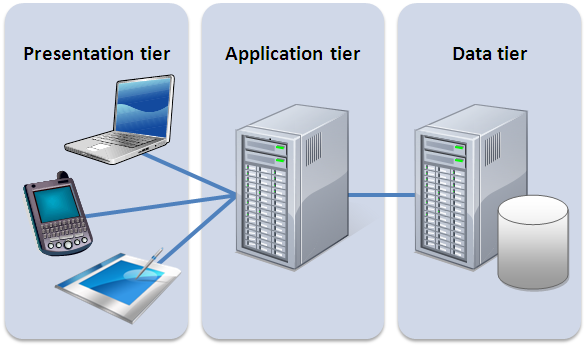
\includegraphics[width=90mm]{obrazky-figures/3vrstva.png}
    
    \caption{Třívrstvá architektura. Převzato z: \cite{threelayer}.}
\end{center}
\end{figure}


\subsection{Architektura klient-server}

Tato architektura se v dnešní době už tolik nevyužívá, protože bývá nahrazována již zmíněnou třívrstvou architekturou. Uvádím ji zde pouze pro představu, jaké jsou mezi nimi odlišnosti. Tato architektura se oproti třívrstvé architektuře skládá pouze ze dvou částí: klienta a serveru. Pokud chce klient vyžívat nějakou službu, kterou server nabízí, připojí se k serveru a následně mezi sebou vzájemně komunikují a posílají si data. Klient posílá požadavky a server následně odpovídá, pro každého klienta vytvoří server relaci. V dnešní době je tato architektura nahrazena právě proto, že klient obsahuje většinu aplikační logiky a aplikace jsou velmi složité, proto rostou nároky na počítače a zařízení obecně. Také kvůli bezpečnosti není v dnešní době architektura vhodná. \cite{clientserver}

Na serveru je dostupná relační databáze, nad kterou server provádí zpracování dotazů. Klient obsahuje aplikační logiku a uživatelské rozhraní pro uživatele. Uživatel posílá požadavky, které klient přeloží do podoby, která je pro server srozumitelná. Poté dostane odpověď od serveru, kterou opět přeloží, tak aby byla srozumitelná pro uživatele a zobrazí mu výsledek v přijatelné podobě. \cite{clientserver}

\begin{figure}[H]
    \begin{center}
    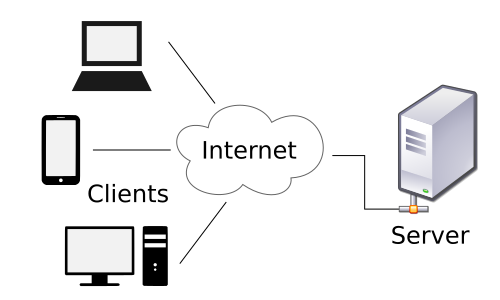
\includegraphics[width=90mm]{obrazky-figures/cliserver.png}
    
    \caption{Architektura klient-server. Převzato z: \cite{clientimage}.}
\end{center}
\end{figure}


\section{Informační systém}

Informační systém lze chápat jako vzájemně propojené informace a s nimi pracující procesy. Můžeme říci, že informace jsou data, pomocí kterých se v systému řídíme a rozhodujeme. Procesy se dají chápat jako funkce, které transformují vstupní údaje na výstupní. Procesy tedy zabezpečují sběr, uložení, přenos a distribuci dat. \cite{is1} 

\begin{figure}[H]
    \centering
    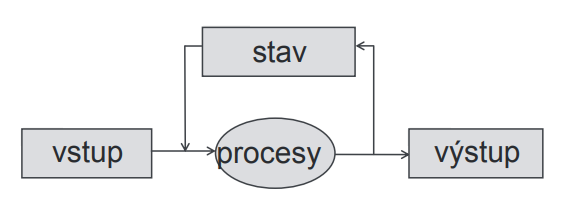
\includegraphics[width=100mm]{obrazky-figures/is.png}
    
    \caption{Schéma informačního systému. Převzato z: \cite{isimage}.} 
    \label{fig:my_label}
\end{figure}


\section{Klasifikace informačních systémů}

 Informační systémy se dají rozdělit podle jejich klasifikace do dvou základních skupin, těmi jsou OLTP a OLAP systémy.

\subsection{OLTP systémy}

Pomocí OLTP(Online Transaction Processing) systémů může uživatel databázového serveru provádět mnoho trasnsakcí online. Mezi tyto transakce patří například vkládání, mazání, dotazování nebo provádění jednoduchých analýz nad daty v databázi. V praxi si tyto transakce můžeme představit například jako  internetové bankovnictví nebo nákupy v e-shopech, jsou to tedy systémy, které využívají uživatelé v běžném životě.
Mezi výhody OLTP patří zejména to, že více uživatelů přistupuje ke stejným datům a provádí nad nimi velké množství transakcí a zároveň zajišťuje integritu dat. Také poskytuje indexované soubory dat. \cite{oltp}

\subsection{OLAP systémy}

Systémy OLAP(Online Analytical Processing) jsou systémy určené pro pokročilé analyzování velkého množství dat. Díky těmto analýzám vznikají reporty a souhrny dat, na jejichž základě se rozhodují manažeři v oblasti řízení firmy, řízení technologických nebo ekonomických procesů. Pro získání analýz pomocí OLAP je zapotřebí vykonat velké množství různých operací, a rozhodně se nejedná o triviální proces. \cite{lacko}

\begin{figure}[H]
    \begin{center}
        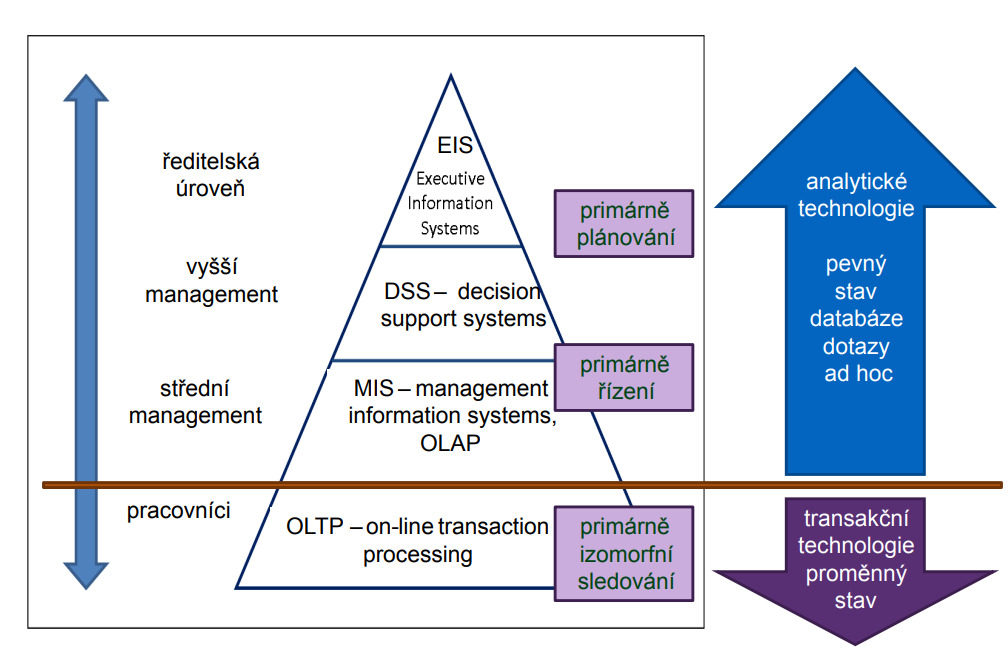
\includegraphics[width=130mm]{obrazky-figures/oltpolap.png}
    \caption{ Klasifikace informačních systémů na základě úrovně rozhodování. Převzato z: \cite{isimage}.}
    \end{center}
\end{figure}

\section{Back-end}

Jedná se o administrační sekci webu, sloužící k administraci obsahu stránek. Tato sekce není běžným uživatelům přístupná. Pro přístup k této části aplikace je totiž vyžadována autorizace. \cite{backend}


\subsection{PHP}

PHP(Hypertext Preprocessor)\footnote{Dostupné z:\url{https://www.php.net/}.} je multiplatformní programovací jazyk pracující na straně serveru. Byl vyvinut Rasmusem Lerdorfem pro vývoj webů. PHP je multiplatformní jazyk, lze ho tedy používat na většině operačních systémů. Zejména se používá pro tvorbu dynamických webových stránek, ale lze ho použít také pro vývoj desktopových aplikací. PHP není příliš náročné pro uživatelská zařízení, proto je v dnešní době velice rozšířené a oblíbené. \cite{php}

PHP má mnoho frameworků pro vývoj webových aplikací, mezi které patří například Laravel, Nette nebo Symfony.

\subsection{Java}

Java\footnote{Dostupné z:\url{https://www.java.com/en/}.} je programovací jazyk, který byl vyvinut firmou Sun Microsystems v roce 1995. Java je vysokoúrovňový programovací jazyk, který podporuje objektově orientované programování. Mezi největší výhody Javy patří to, že je multiplatformní a vysoce zabezpečený. \cite{java}
Java má také mnoho frameworků, mezi ty patří například Spring, JSF nebo GWT.

\subsection{Python}


Python\footnote{Dostupné z: \url{https://www.python.org/}.} je vysokoúrovňový, objektově orientovaný a interpretovatelný programovací jazyk, který je v dnešní době velice populární. Jeho největší výhodou je určitě to, že je velice jednoduchý, přehledný a obsahuje méně syntaktických konstrukcí než jiné jazyky, proto je také vhodný pro začátečníky s programováním. Je také dynamicky typovaný a nabízí velké množství knihoven, které lze využít. \cite{python}

Python také nabízí různé frameworky, těmi nejznámějšími jsou: Django, Pyramid nebo Flask.

\section{Front-end}

Front-end je grafický výstup webové aplikace, jedná se tedy o sekci aplikace, kterou vidí uživatel. Proto by měl být zvláště kladen důraz na to, aby byl frontend dosatečně přehledný, uživatelsky přívětivý a jednoduchý.

\begin{figure}[H]
    \centering
    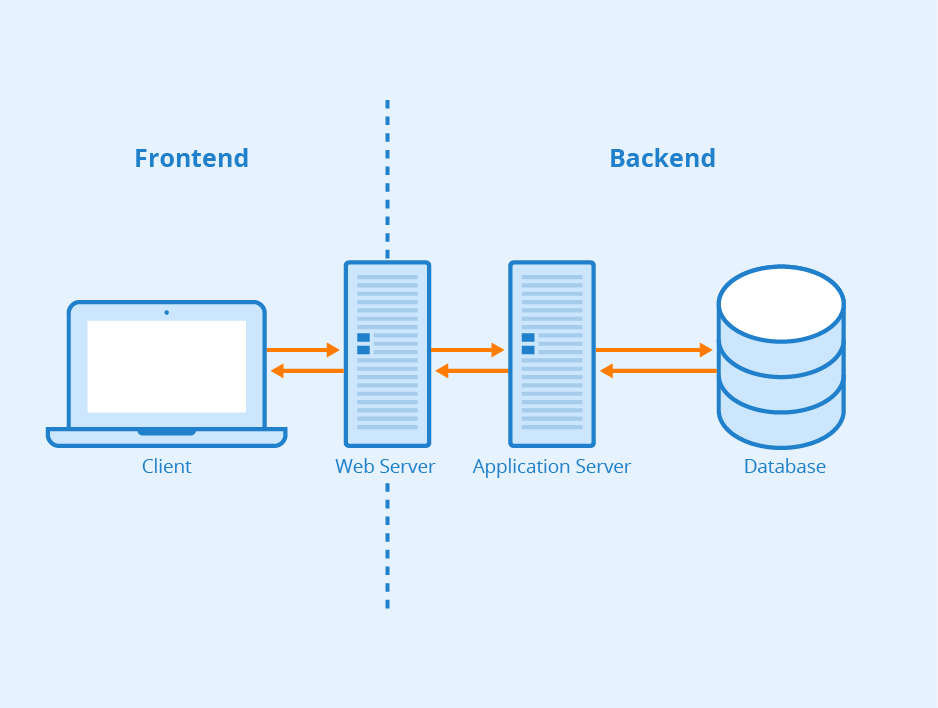
\includegraphics[width=100mm]{obrazky-figures/Frontend.png}
    
    \caption{Vztah backendu a frontendu Převzato z: \cite{frontbackimage}.}
\end{figure}



\subsection{HTML}

HTML(HyperText Markp Laguage) je značkovací jazyk používaný k tvorbě obsahu webových stránek. Jeho strukturu tvoří html tagy, které mohou být párové nebo nepárové a mohou obsahovat další atributy. Tagy obalují text, který je pak formátován podle toho, který tag jej obklopuje. \cite{html}

Celá struktura html dokumentu je mezi tagy \texttt{<html>} a \texttt{</html>}, dále musí obsahovat tagy \texttt{<head>} a \texttt{</head>}, tyto tagy označují hlavičku dokumentu, ta obsahuje metadata, například titulek nebo odkaz na CSS soubor. Samotný obsah dokumentu se píše mezi tagy \texttt{<body>} a \texttt{</body>}. \cite{html}

\subsection{CSS}

Jazyk CSS(Cascading Style Sheets) byl vytvořen v roce 1994, je to jazyk sloužící pro popis vzhledu webové stránky pro jazyk HTML. Pomocí CSS můžeme například měnit barvu a styl písma nebo měnit zarovnání textu a rozložení celé stránky. \cite{css}

CSS styl můžeme přidat do HTML dokumentu několika způsoby: \cite{css}

\begin{itemize}
  \item{Zapsání pravidla přímo do HTML elementu.}
  \item{Přidání elementu \texttt{<style>} v elementu \texttt{<head>} v HTML dokumentu.}
  \item{Nejčastěji se využívá zadání odkazu na externí CSS soubor v elementu <head>.}
\end{itemize}

Pro použití CSS musíme zadat pravidlo, které se skládá ze selektoru a deklarace. Pomocí selektoru se pozná na jaký HTML element se má pravidlo použít, může se jednat přímo o html tag, třídu nebo identifikátor. Třídu vytvoříme tak, že do elementu přidáme atribut \texttt{class}(příklad: class="trida") a jeho název. V případě, že se jedná o identifikátor, zadáme klíčové slovo \texttt{id} a název(příklad: id="identifikator"). \cite{css}

Příklad zapsání pravidla CSS:

\begin{itemize}
  \item{Nastavení fontu pro html element p: \texttt{p \{font-family: "Times New Roman";\}}}
  \item{Nastavení červené barvy písma pro třídu: \texttt{.trida: \{color: red;\}}}
  \item{Nastavení velikosti písma 20 pro identifikátor: \texttt{\#identifikator \{font-size: 20;\}}}
\end{itemize}


\subsection{Java-script}

Javascript\footnote{Dostupné z:\url{https://www.javascript.com/}.} je objektově orientovaný multiplatformní jazyk, který byl vytvořen v roce 1995. Syntaxe java-scriptu patří do stejné rodiny jako například Java nebo C. Je to dynamicky typovaný jazyk. Je využíván zejména proto, že pomocí něj můžeme měnit obsah webové stránky u uživatele. To nám otevírá možnost tvořit dynamické menu a další komponenty, které umožňují ušetřit místo na stránce když jsou zavřené a po najetí myší se otevřou. \cite{javascript1}

Mezi největší výhody patří zejména to, že je java-script rychlý a rozšiřitelný. Na druhou stranu může kvůli němu dojít k ohrožení bezpečnosti klienta. \cite{javascript2}

\section{Databáze}

Databáze je softwarový systém, sloužící
pro uchovávání dat při tvorbě webových aplikací a informačních systémů a následné správě těchto dat. Databáze běží na serveru a webové aplikace si z nich stahují data, které se poté zobrazují na webových stránkách prostřednictvím  webového prohlížeče. Existuje několik typů databází, mezi ty patří například: relační, hierarchické, síťové nebo objektové databáze. \cite{db1} V této práci pracuji s relační databází.


 SŘBD(Systém řízení báze dat) je univerzální označení pro software, který zprostředkovává komunikaci mezi aplikacemi a uloženými daty. SŘBD umožňuje provádět s daty následující operace: spouštění dotazů, ukládání, mazání a aktualizaci. \cite{db2} 

\subsection{Relační databáze}

Relační databáze se skládá z tzv. relací, které reprezentují databázové tabulky. Tyto tabulky mohou být navzájem propojeny. Každá tabulka je definována záhlavím a tělem. Sloupce tabulky představují atributy a řádky tabulky reprezentují záznamy v tabulce. \cite{relacnidb}

V relačních databázích máme primární a cizí klíče. Primární klíč je atribut jednoznačně identifikující záznamy a cizí klíč vytváří vztahy mezi tabulkami, tím že odkazuje z jedné tabulky na primární klíč jiné tabulky. \cite{relacnidb}


\subsection{MySQL}

MySQL\footnote{Dostupné z: \url{https://www.mysql.com/}.} bylo vytvořeno švédskou firmou MySQL AB v roce 1995, v dnešní době  jej vlastní společnost Oracle Corporation, jedná se o jeden z nejpoužívanějších databázových systémů vůbec. MySQL uplatňuje relační databázový model, data tedy ukládá do tabulek, kde každá tabulka reprezentuje jednu entitu dat. Komunikace s databází probíhá pomocí dialektu jazyka SQL, který má určitá rozšíření oproti klasickému SQL. \cite{mysql1} 

Jedná se o multiplatformní databázi, takže je přenositelná mezi více různými platformami. MySQL je poskytováno zdarma a je velice rychlé a jednoduché, nabízí však omezený počet funkcí. Kromě verze zdarma, existuje také placená verze, která poskytuje velké množství funkcí navíc. Pro práci s databází je v této práci využit velmi populární databázový řídící systém PHPMyAdmin, který umožňuje jednoduchou správu databáze prostřednictvím webového rozhraní. \cite{mysql2} 


\subsection{Další populární databázové systémy }

Dalšími populárními databázovými systémy ve světě jsou \cite{dbpopular}: 

\begin{itemize}
\item Oracle database – Multiplatformní databázový systém vyvíjen firmou Oracle, který umožňuje pokročilé zpracování dat a nabízí velmi vysoký výkon.
\item Microsoft SQL Server - Databázový systém vytvořen firmou Microsoft v roce 1989. Opět nabízí vysoký výkon. 
\item Postgres SQL - Vydáno v roce 1996 firmou PostgreSQL Global Development Group.

\end{itemize}


\chapter{Získávání znalostí dat}
\label{zzn}

Tato kapitola pojednává o problematice získávání znalostí dat. Jsou zde popsány všeobecné základy, ale také informace zaměřující se na různé druhy dolovacích metod.

\section{Úvod}

Získávání znalostí dat(data-mining) je proces, při kterém získáváme zajímavé modely dat a vzorů z velkých objemů dat. Tyto modely a vzory reprezentují znalosti získané z dat. Získávání znalostí není triviální, znamená to tedy, že tyto znalosti nejsou na první pohled v databázi viditelné, nebo nestačí na jejich získání použít pouze SQL dotaz, ale je potřeba využít složité postupy, které zahrnují například použití netriviálních matematických vzorců.
Získávání znalostí dat se rozmohlo zejména v dnešní době a několika posledních letech, kdy máme obrovský objem dat a je zapotřebí přeměnit tyto data na užitečné informace a znalosti. Ty je pak možné využívat v mnoha různých oblastech. \cite[Kapitola~1]{Kamber}


\subsection*{Proces získávání znalostí}
Při získávání znalostí se řídíme určitým postupem, který se skládá z několika kroků, těmi jsou: \cite[Kapitola~1]{Kamber}

\begin{enumerate}
  \item{Čištění dat – Pokud chybí nějaká data, musíme se se ztrátami vypořádat, také odstranit šum a řešit různé nekonzistence dat.}
  \item{Integrace dat – Integrujeme data, které pochází z několika různých zdrojů.
Čištění i integrace jsou obvykle řešeny v jednom kroku, v takovém případě ukládáme data do datového skladu.  Je to  zapříčiněno tím, že data po čištění musíme rovnou někam ukládat. Data z různých zdrojů jsou také většinou nekonzistentní.
}
  \item{Výběr dat -  V tomto kroku vybíráme data, která jsou relevantní. Vybíráme tedy z jedné tabulky určité sloupce(atributy).}
  \item{Transformace dat – Data musíme transformovat do podoby, ze které je možno provádět dolování. Jedná se například o agregaci nebo sumarizaci.}
  \item{Dolování dat – Jak již název napovídá, jedná se o nejdůležitější krok, při kterém dochází při aplikaci určité metody a konkrétního algoritmu k extrakci vzorů z dat.}
  \item{Hodnocení modelů a vzorů – Identifikujeme zajímavé vzory, které budou nejužitečnejší.}
  \item{Prezentace znalostí – Poslední krok, při kterém prezentujeme získaná data uživateli.}
\end{enumerate}

\begin{figure}[H]
    \begin{center}
        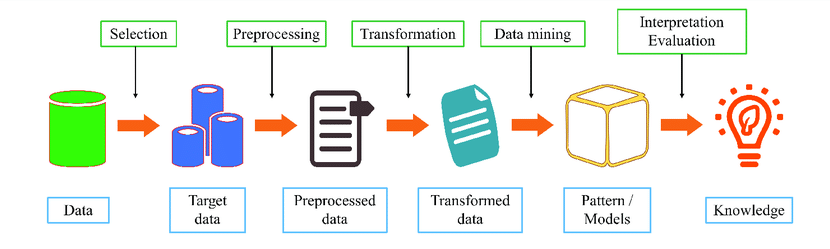
\includegraphics[width=130mm]{obrazky-figures/proces-mining.png}
    
        \caption{Proces dolování dat. Převzato z: \cite{datamining}.}
    \end{center}
    
\end{figure}


\subsection*{Typy dolovacích úloh}
Typ dolovací úlohy určujeme podle toho, který model dat chceme po dolování získat. Dolovací úlohy můžeme rozdělit do dvou základních skupin, těmi jsou: \cite[Kapitola~1]{Kamber}

\begin{enumerate}
  \item{Deskriptivní – Jedná se o obecné vlastnosti analyzovaných dat. Například zjištění častých společných nákupů, pomocí analýzy nákupního košíku.}
  \item{Prediktivní – Provádí dedukci pro předpověď budoucího chování na základě analýzy dat současných. Příkladem je klasifikace, pomocí které můžeme určit, zda je vhodné určité osobě poskytnout úvěr na základě jeho platu a dalších aspektů.}

\end{enumerate}

\section{Předzpracování dat pro dolování}
Data je potřeba nějakým způsobem předzpracovat, protože databáze standartně nejsou ve stavu, abychom z nich rovnou mohli dolovat. V databázích jsou často data, která jsou zašuměná, nekonzistentní, nebo dokonce určitá data chybí. Tato neočištěná data by nás mohli dovést při dolování ke zkresleným nebo chybným závěrům.
Kvalita dat se všeobecně hodnotí podle několika kritérií. Data by měla co nejpřesněji odpovídat realitě, kterou modelují a musí být aktuální. Měla by být úplná, to znamená mít dostatečný počet hodnot(úplnost do hloubky) a zároveň dostatek potřebných atributů(úplnost do šířky). Data musí být také konzistentní a jejich věrohodnost musí být co nejvyšší. Také se řeší, jak snadno jsou data dostupná a hodnoty by měly být snadno interpretovatelné. \cite[Kapitola~3]{Kamber} 


Pro dolování platí již zmíněná kritéria také, ale nekvalita dat v souvislosti s předzpracováním se nejčastěji týká těchto problémů: \cite[Kapitola~3]{Kamber}

\begin{itemize}
\item Nekompletní data – Některé hodnoty v databázi mohou chybět, to může být zapříčiněno několika důvody, například při zadávání dat byla položka označena jako nepovinná, položka mohla být zadána chybně nebo došlo k nějaké poruše. Hodnota také mohla být nekonzistentní s ostatními hodnotami a tak byla zrušena.
\item Zašuměná data – atributy obsahují odlehlé nebo nesprávné hodnoty. Může se jednat například o hodnotu venkovní teploty o hodnotě 1000°C.  Příčinou může být například chyba při sběru dat.
\item Nekonzistentní data – Může dojít k redundanci dat, pokud použijeme data z několika různých zdrojů. Nekonzistence mohou být v pojmenování, kódování nebo formátech a dalších. Redundance ale může nastat i u dat z jednoho zdroje, například při špatném návrhu databáze. 

\end{itemize}

\subsection*{Hlavní úlohy předzpracování: \cite[Kapitola~3]{Kamber}} 

\begin{enumerate}
  \item{Čištění dat – Při tomto kroku se snažíme odstranit odlehlé a chybějící hodnoty a řešit nekonzistence. Pokud bychom měli dolovat z nekvalitních dat, mohl by být ovlivněn dolovací algoritmus a my bychom mohli dostat nespolehlivé výsledky.}
  \item{Integrace dat -  Integrujeme data z různých datových zdrojů.}
  \item{Transformace dat – Data je nutné transformovat do tvaru vhodného pro řešení dané dolovací úlohy. Jedná se o agregaci a normalizaci. }
  \item{Redukce dat - V tomto kroku se snažíme zredukovat objem dat. I menší redukce je velice nápomocná a usnadní mnoho práce při dolování. Patří sem například redukce počtu hodnot a redukce dimenzionality.}
  \item{Diskretizace dat – Jedná se také o redukci dat, ale má zvláštní význam, a to takový, že se redukují počty hodnot atributů. Týká se hlavně spojitých dat.}

\end{enumerate}


\section{Klasifikace a predikce}

V této podkapitole jsou popsány základy klasifikace a predikce, také jsou uvedeny příklady jejich metod.

\subsection{Klasifikace}

Klasifikace je proces, díky kterému jsme  schopni data přiřadit do určitých tříd na základě jejich vlastností. Jako příklad pro klasifikaci může být uvedena banka, do které zákazníci přijdou pro úvěr. Pomocí klasifikace jsme schopni rozdělit zákazníky do dvou skupin na základě jejich vlastností, například na základě jejich platu, hypotéce, majetku a další. První skupina budou zákazníci, kterým bude úvěr schválen a do druhé skupiny budou patřit zákazníci, u kterých by bylo riziko úvěru příliš vysoké a úvěr nedostanou. \cite[Kapitola~8]{Kamber}

\subsection*{Fáze klasifikace}

První fáze klasifikace se nazývá fáze učení. V této fázi jsou vybrány vzorky dat z databáze, množinu vybraných dat nazýváme trénovací množinou. Vzorky dat dále slouží jako vstup pro klasifikátor, u těchto vzorků musíme předem vědět do jaké třídy je zařadit. Klasifikátor poté zjistí, jaká jsou klasifikační pravidla, které poté slouží pro klasifikaci objektu do dané třídy. \cite[Kapitola~8]{Kamber}


Druhá fáze je testovací. V této fázi vybereme vzorky dat, u kterých víme, do které třídy je zařadit a neměly by být vybrány z trénovací množiny. Tato množina dat se nazývá trénovací množina. Data se poté zařazují do tříd pomocí klasifikátoru, který už ví z předchozí fáze, do jaké třídy data zařadit. Po zařazení dat se procentově určí, v kolika případech byla provedena správná klasifikace a poté se rozhodne, jestli může být klasifikátor běžně využíván v praxi. \cite[Kapitola~8]{Kamber}

\paragraph{Metody Klasifikace} 

\begin{itemize}
  \item{Rozhodovací strom}
  \item{Bayesovská klasifikace}
  \item{Klasifikace pomocí neuronových sítí}

\end{itemize}

\subsection{Predikce}
Predikce je proces, pomocí kterého lze přiřazovat hodnoty datům, které mají spojitý charakter. Jako příklad lze uvést určení platu pracovníka na základě jeho aktuálního platu. \cite[Kapitola~8]{Kamber}

\paragraph{Metody predikce} 

\begin{itemize}
  \item{Lineární jednoduchá regrese}
  \item{Lineární vícenásobná regrese}
  \item{Nelineární regrese}

\end{itemize}



\section{Dolování asociačních pravidel a frekventovaných množin}

Asociační pravidla nám ukazují vztahy mezi položkami ve vzorku dat. Můžeme s jejich pomocí například určit, jaké položky si v obchodě často kupují zákazníci společně a na základě tohoto zjištění může prodejce vytvářet různé akční nabídky nebo mít vystavené tyto produkty poblíž sebe.



Při získávání znalostí dat existují dvě metriky, těmi jsou podpora a spolehlivost. Podpora určuje v kolika procentech byly dvě položky koupeny společně v rámci jedné transakce. Druhá z nich je spolehlivost, která určuje procento zákazníků, kteří si někdy koupili položku a poté si v rámci jiné transakce koupili druhou.

Při získávání asociačních pravidel jsou důležité 2 kroky. Prvním z nich je nalezení frekventovaných množin, což jsou ty položky, které splňují podmínku minimální podpory. Druhým krokem je poté již generování silných asociačních pravidel z dříve nalezených frekventovaných množin. U těchto pravidel musí být splněna podmínka minimální podpory a také podmínka minimální spolehlivosti. \cite[Kapitola~6]{Kamber}

\subsection{Typy asociačních pravidel}

Existuje několik různých typů asociačních pravidel. Samotná asociační pravidla se klasifikují podle několika kritérií: \cite[Kapitola~6]{Kamber}

\textbf{Podle typu hodnot v pravidlech} - Podle tohoto kritéria rozlišujeme booleovská a kvantitativní asociační pravidla. O booleovská asociační pravidla se jedná, pokud se zajímáme pouze o přítomnost nebo nepřítomnost položky, naopak o kvantitativní asociační pravidla se jedná pokud tyto pravidla popisují asociace mezi kvantitativními položkami nebo atributy. \cite[Kapitola~6]{Kamber} 

\textbf{Podle dimenzí obsažených v pravidlech} - Asociační pravidla se dají rozdělit podle počtu obsažených dimenzí. Jednodimenzionální asociační pravidla jsou booleovská pravidla, protože obsahují pouze jednu dimenzi, konkrétně v již zmíněném příkladu dimenzi, která určuje, zda zboží bylo zakoupeno či nikoliv. Vícedimenzionální pravidla jsou pravidla kvantitativní, protože kromě dimenze, zda bylo zboží zakoupeno, obsahují také další dimenze.

\textbf{Podle úrovní abstrakce} - Existují víceúrovňová asociační pravidla. Některé metody mohou získávat asociační pravidla nad těmito pravidly z různých úrovní abstrakce. \cite[Kapitola~6]{Kamber}

\subsection{Algoritmus apriori}


Apriori je nejjednodušší varianta získávání asociačních pravidel. Apriori doluje jednoúrovňová asociační pravidla, tedy zjišťuje pouze jednu dimenzi, konkrétně zda se položka vyskytuje v transakci nebo ne.
Tento algoritmus využívá předchozí znalost o již získaných frekventovaných množinách. V každé iteraci jsou získané frekventované k-množiny použity k vygenerování (k+1) množin, je tedy nutné projít databázi v každé iteraci, z tohoto důvodu se nejedná o nejrychlejší metodu.

Pro vyšší efektivitu je využívána vlastnost Apriori, která říká, že každá podmnožina frekventované množiny musí být frekventovaná také. Vlastnost Apriori vychází z faktu, že přidání prvku do množiny nemůže způsobit vzrůst její podpory. \cite[Kapitola~6]{Kamber}

Algoritmus Apriori pracuje následujícím způsobem: \cite[Kapitola~6]{Kamber}


\begin{enumerate}
  \item Při první iteraci projdeme celou databázi a spočítáme podporu pro každou položku. Množina C\textsubscript{1} bude obsahovat všechny tyto položky.
  \item  Určíme minimální podporu, poté nalezneme množinu L\textsubscript{1}, ta bude tvořena položkami C\textsubscript{1}, které splňují minimální podporu.
  \item Dalším krokem je vygenerování C\textsubscript{2} při spojení množin z L\textsubscript{1}.
  \item Vypočítá se podpora kandidátů z C\textsubscript{2} a odstraní se kandidáti, kteří nesplňují minimální podporu. Výsledkem je množina L\textsubscript{2}.
  \item Vygeneruje se C\textsubscript{3} z množiny L\textsubscript{2} tím, že se vytvoří množiny po třech prvcích. Z C\textsubscript{3} můžeme odstranit podmnožiny, které nejsou frekventované v L\textsubscript{2}.
  \item Tímto způsobem pokračujeme dál a zvyšujeme počty prvků v množinách C\textsubscript{k}. Jakmile je nějaká množina C\textsubscript{k} prázdná, můžeme algoritmus ukončit a výsledkem je množina L\textsubscript{k-1}.
\end{enumerate}

\subsection{Metoda FP-stromu}

Algoritmus Apriori může mít problém s generováním kandidátů u velkých databází, protože obsahují velké množství dat. Tento problém se dá řešit metodou vzrůstu frekventovaných množin u které se nejdříve databáze zkomprimuje do struktury nazvané strom frekventovaných množin(FP-strom). Poté se strom rozdělí do podmíněných FP-stromů, ty jsou vytvořeny pro všechny frekventované položky. Z těchto stromů poté získáme frekventované množiny.
Efektivitu algoritmu Apriori mohou také zvýšit další úpravy, například: hešovací přístup, redukce transakcí, vzorkování nebo rozdělení dat. \cite[Kapitola~6]{Kamber}


\section{Shluková analýza}

Shlukování rozděluje objekty na základě jejich podobnosti do tříd(clusterů). Výsldkem jsou třídy, které obsahují velice podobné objekty a jsou velice odlišné od objektů z jiných tříd. K určení podobnosti objektů se často využívají vzdálenostní funkce. \cite[Kapitola~10]{Kamber}

Shlukovací metody mají mnoho různých vlastností, většinou jsou na ně ale kladeny tyto požadavky: \cite[Kapitola~10]{Kamber}

\begin{itemize}
  \item{Škálovatelnost}
  \item{Schopnost zpracovávat různé typy atributů}
  \item{Tvorba shluků různého tvaru}
  \item{Vyrovnání se s šumem}
\end{itemize}



Je mnoho druhů shlukovacích metod. Konkrétní shlukovací metoda se zvolí na základě typu analyzovaných dat a na konkrétním účelu aplikace. Shlukovací metody se dělí následovně: \cite[Kapitola~10]{Kamber}

\begin{itemize}
  \item{Metody založené na rozdělování - Metody, které rozdělují objekty do tříd, přičemž každá třída musí obsahovat alespoň jeden objekt a každý objekt může patřit pouze do jedné třídy.}
  \item{Hierarchické metody - Metody vytvářející hierarchický rozklad dané množiny objektů, vzniká tak strom shluků.}
  \item{Metody založené na hustotě - Metody, které považují za shluky oblasti s velkou hustotou objektů, které jsou odděleny oblastmi s malou hustotou výskytu objektů(šum) v datovém prostoru.}
  \item{Metody založené na mřížce - Tyto metody využívají datovou strukturu v podobě víceúrovňové mřížky. Prostor objektů rozdělují na konečný počet buněk.}
  \item{Metody založené na modelech - Tyto metody se snaží optimalizovat shodu mezi matematickým vzorcem a datovou množinou. Snaží se tedy nalézt shluky, které co nejvíce odpovídají danému modelu.}
\end{itemize}


\section{Datové sklady a OLAP technologie}

V této podkapitole jsou stručně popsány datové sklady a jejich porovnání s relačními databázemi. Dále jsou zde popsány základy technologie OLAP, schémata OLAP a operace.

\subsection{Datový sklad}

 Datový sklad je zvláštní typ databáze, který primárně slouží pro analýzu dat v oblasti, kde slouží jako podklady pro manažerské rozhodování. \cite{sklad}
 Datový sklad může být zkonstruován poté, co jsou data očištěna a integrována. Jedná se o velmi důležitý krok v předzpracování, proto aby později mohlo být uskutečněno získávání znalostí. \cite[Kapitola~4]{Kamber}
 
\subsection*{Rozdíl mezi běžnou relační databází a datovým skladem}

V relační databázi se obvykle snažíme o co nejmenší redundanci ukládaných dat. Redundance dosahujeme vnitřním provázáním jednotlivých funkčních celků nebo normalizací. Datový sklad se na rozdíl od relační databáze snaží o jasnou vnitřní separaci jednotlivých funkčních celků, jejíž výsledkem je poté struktura, kterou mohou uživatelé lépe číst, avšak za cenu zvýšených nároků na paměťový prostor. Pokud popisujeme strukturu datového skladu, popisujeme ji jako multidimenzionální strukturu uložených dat. \cite{sklad}

\subsection{Multidimenzionální datový model}

Data, nad kterými jsou prováděny OLAP operace jsou zobrazeny ve formě datové kostky, ta nám umožňuje data vnímat jako vícerozměrná. Datová kostka je definována dimenzemi a fakty.

Dimenze mohou být entity nebo pohledy. Záznamy v nějakém obchodě mohou být ukládány vzhledem k prodávanému zboží, místě prodeje, dodavateli a času, kdy byly prodány. Každé této dimenzi budou přiřazeny tabulky dimenzí, které tyto dimenze popisují. Například tabulka dimenze dodavatele může mít tyto atributy: jméno, adresa, telefon a další.

Dále jsou v multidimenzionálním datovém modelu tabulky faktů. Fakta jsou numerické měrné jednotky, představují množství, na jehož základě poté analyzujeme vztahy mezi dimenzemi. Kromě fakt obsahuje tabulka faktů také cizí klíče do dimenzí. \cite[Kapitola~4]{Kamber}

\subsection*{Schémata představující dimenzionální databáze}

Narozdíl od OLTP systémů, kde se pro jejich modelování využívají ER-diagramy se u datových skladů používají multidimenzionální modely. \cite[Kapitola~4]{Kamber}

\begin{itemize}
    \item{Schéma hvězdy - Jedná se o nejběžnější schéma. V tomto schématu se nachází tabulka faktů, což je centrální tabulka obsahující velké množství dat bez redundance. Kromě této centrální tabulky je v tomto schématu množina tabulek dimenzí a každá z nich uchovává v rámci atributů informace o jedné dimenzi.}
    
    \item{Schéma sněhové vločky - Toto schéma je obdobné jako schéma hvězdy s tím rozdílem, že jsou některé tabulky dimenzí normalizovány, což znamená, že jsou vytvořeny nové tabulky. Největší výhodou tohoto schématu je velká úspora místa z důvodu snížení redundance. Avšak nejvíce prostoru zabere samotná tabulka faktů, což znamená, že celková úspora není tak velká, jak se původně mohlo zdát. Toto Schéma se příliš v praxi nevyužívá z důvodu náročnosti vykonávání dotazů. Mezi tabulkami je totiž nutné provést mnoho spojení.}
    
    \item{Schéma souhvězdí - Toto schéma se využívá, pokud aplikace vyžaduje více než pouze jednu tabulku faktů, které sdílejí některé tabulky dimenzí. Tento model můžeme vnímat jako kolekci hvězd.}
\end{itemize}

\subsection*{OLAP operace v multidimenzionálních datech}

Na multidimenzionální data můžeme pohlížet hned několika různými pohledy, z důvodu, že každá dimenze obsahuje hned několik úrovní abstrakcí. Proto abychom těmito pohledy mohli na data nahlížet, nejběžnější operace jsou uvedeny zde: \cite[Kapitola~4]{Kamber}

\subsection*{Roll-Up}

Tato operace provede na datové kostce agregaci. Jinými slovy se v jedné z hierarchií posuneme o úroveň výše. Například data v kostce po provedení této operace nebudou seskupena podle čtvrtletí, ale podle celých let.

\subsection*{Drill-down}

Tato operace je pravým opakem operace roll-up. Po provedení této operace se posuneme v jedné hierarchii o úroveň níže a dostaneme tak detailnější pohled. 

\subsection*{Slice \& Dice}

Operace Slice \& Dice provede nad jednou dimenzí selekci dat. Výsledkem této operace je podkostka s daty splňující nějakou podmínku.

\subsection*{Rotate}

Operace Rotate(někdy nazývaná Pivot) je vizualizační operace. Mění datové osy za účelem jiné prezentace dat kostky.




\chapter{Analýza a požadavky na systém}
\label{analysis}

První krok, který je zapotřebí uskutečnit při tvorbě informačního systému je krok, který předchází návrhu systému, jedná se o důkladnou specifikaci požadavků od zákazníka, pro kterého informační systém vytváříme. Musíme přesně zjistit, kdo všechno bude se systémem pracovat, a jaké akce bude chtít v systému vykonávat. Naším úkolem je tyto požadavky analyzovat a zjistit, zda je vůbec možné všem těmto požadavkům vyhovět, pokud ne, je zapotřebí se zákazníkem najít určitý kompromis, který je možné implementovat.

V této kapitole jsou popsány požadavky na informační systém od zákazníka. Informační systém budou používat uživatelé, kteří budou mít jednu ze tří rolí: admin, zákazník, zaměstnanec.

\section{Zákazník}

Jako zákazník je chápána jakákoliv firma, která se zaregistruje do informačního systému. Firma se může zaregistrovat sama, nebo může požádat admina a ten firmu zaregistruje sám. Firma při registraci zadá svoje údaje do registračního formuláře, je nutné zadat login a heslo pomocí něhož se bude později do systému přihlašovat. Po založení účtu si může každá firma zadat do systému neomezený počet kontaktních osob, které mohou zaměstnanci nebo admin poté kontaktovat pokud bude třeba. Zákazník si poté může své kontaktní osoby zobrazit a také měnit jejich údaje, nebo je úplně odstranit. Kontaktní osobu může k firmě přidat také admin.

Zákazník si po registraci může libovolně měnit svoje údaje, které zadal při registraci a také si může změnit heslo. Tuto možnost má také admin, pokud by zákazník zapomněl svoje heslo, může požádat admina a ten mu heslo změní.




\section{Zaměstnanec}

Účet zaměstnance je vytvořen adminem poté, co je zaměstnanec přijat do firmy. Poté se zaměstnanec do systému přihlašuje pomocí svého emailu a hesla, které byly zadány při registraci. Zaměstnanec si pak může heslo a své ostatní údaje libovolně měnit, pokud je potřeba. Každý zaměstnanec má ve firmě konkrétní pozici, na kterou byl přijat. Podle této pozice je přidělen na oddělení a je mu přidělena funkce. V systému jsou zaměstnanci, kteří mohou mít jednu z následujících funkcí: 



\begin{itemize}
  \item{Míchač}
  \item{Skladník}
  \item{Balič}
\end{itemize}

Podle určité funkce, kterou zaměstnanec ve firmě zastává poté provádí práci, avšak v systému je umožněno, aby například míchač mohl naskladnit zboží, v případě, že by zaměstnanec musel nahradit jiného zaměstnance v případě jeho absence. 

\section{Manipulace s objednávkami}

Objednávku může vytvořit zákazník, nebo ji pro konkrétního zákazníka může vytvořit admin. Každá objednávka má termín, do kterého má být vyřízena. Po založení objednávky je automaticky termín nastaven na datum, které je za týden od data vytvoření objednávky, tento termín poté zákazník může změnit. Termíny objednávek se automaticky objeví v google kalendáři jako celodenní událost, ta nese název, ve kterém je obsaženo ID objednávky. Pokud zákazník nebo admin tento termín změní, nebo je objednávka odstraněna, projeví se tato změna také v google kalendáři. Pokud by zákazník zvolil termín, ve kterém není možné objednávku vyřídit, ozval by se mu zaměstnanec a dohodl se s ním na kompromisu. Objednávku může zákazník nebo admin měnit a také ji může úplně odstranit.

Každá objednávka je v nějakém stavu, objednávky v tomto systému mohou mít jeden z následujících stavů:

\begin{itemize}
  \item{Založeno}
  \item{Namícháno}
  \item{Zabaleno}
  \item{Vyřízeno}
\end{itemize}

Po založení je objednávka automaticky ve stavu založeno. Stav objednávky dále mění zaměstnanci firmy, tento stav poté mohou sledovat zákazníci a  mohou tak odhadnout, za jak dlouho objednávka bude přibližně připravena.

Admin a zaměstnanec si mohou zobrazit všechny objednávky, vidí jejich informace a po rozkliknutí vidí jejich obsah. Zákazník si může zobrazit pouze svoje objednávky, tedy ty, které si sám vytvořil nebo mu ji vytvořil admin.


\subsection{Práce na objednávce}

U každé objednávky je umožněno zaměstnanci označit práci na objednávce, kterou provedl. Zaměstnanec může označit dva druhy práce na objednávce: mícháni a zabalení. Zaměstnanec má po přihlášení přístup k přehledu všech svých vykonaných činností na objednávkách, ale nevidí provedenou práci ostatních, k tomu má přístup pouze admin. 


\section{Položky v objednávce}

Každá objednávka se skládá z několika položek. Položky do objednávky může přidávat admin, nebo zákazník, který objednávku vytvořil. Položky lze různě upravovat, měnit jejich množství nebo je úplně odstranit. U každé položky je možné vybrat konkrétní balení.


\section{Produkty}

Položky, které se do objednávky přidávají jsou produkty. V systému existují dva základní druhy produktů, konkrétně originální a míchané. Každý produkt je identifikován jednoznačným kódem, pomocí jehož prvního písmena poznáme zda se jedná o originální produkt (kód začíná znakem "O") nebo míchaný produkt (kód začíná znakem "M"). Produkty do systému přidává pouze admin a také jedině on je může upravovat nebo mazat. Zákazníci a zaměstnanci si mohou zobrazit jejich seznam. Produktů je na skladě logicky omezené množství, toto množství při přidání produktu do systému zadá admin, poté ho mohou doplňovat zaměstnanci nebo také znovu admin. Každý produkt spadá do jednoho odvětví, v systému mohou produkty spadat do těchto odvětví:

\begin{itemize}
    \item{Barva} 
    \item{Lak} 
    \item{Tmel} 
    \item{Mořidlo} 
\end{itemize}



\subsection{Originální produkty}

Originální produkty jsou produkty, které jsou dodány dodavatelem do firmy a jsou pouze dále přeprodávány ve stejné podobě jako byly doručeny. Tyto produkty do systému přidává admin, který je také potom může měnit, nebo úplně odstranit ze systému. 

Každý originální produkt je dodán jedním dodavatelem. Firma odebírá od několika dodavatelů, o kterých jsou v systému vedeny informace, tyto dodavatele do systému opět přidává, mění a odstraňuje pouze admin. 

\subsection{Recepty míchaných produktů}

Ve firmě se prodávají míchané produkty, to jsou produkty, které firma sama připravuje z originálních produktů, které jim dodal jiný dodavatel. Každý tento produkt má určený recept, podle kterého se produkt míchá. Tento recept zadává do systému pouze admin, také pouze on tento recept může upravovat. Zaměstnanci si tyto recepty zobrazí a podle nich míchají produkty. 


\subsection{Balení produktů}

Každý produkt objednávky musí být nějak zabalen, aby byl bezpečně doručen. Pokud zákazník neurčí jak chce položku zabalit, zaměstnanec položku zabalí podle vlastního uvážení. Pokud chce zákazník zabalit pokožku podle svých konkrétních požadavků, vybere si v systému z nabízených nádob a také vybere jejich počet. Zákazníkovi je dokonce umožněno nechat si jednu položku zabalit do více různých nádob. 

V systému jsou dva typy nádob, těmi jsou: kanystry a plechovky. Každá nádoba má určený objem v litrech. Tyto nádoby do systému zadává, mění a odstraňuje pouze admin. Stejně jako u produktů má každá tato nádoba omezený počet kusů na skladě a je tedy nutné, aby ji zaměstnanec nebo admin naskladňovali. 


\section{Admin}

Admin je nejdůležitější rolí systému. V systému může být více adminů, nové adminy může přidávat pouze jiný admin. Po vytvoření přístupu se admin přihlašuje pomocí emailu a hesla. Adminovi je umožněno provádět veškeré činnosti, které mohou provádět zaměstnanci a zákazníci. Navíc mohou přidávat do systému nové produkty, balení, oddělení nebo registrovat nové dodavatele, kteří do firmy dodávají produkty.


\section{Diagram případů užití}
Diagram případů užití(Use Case Diagram) ukazuje chování systému z pohledu samotného uživatele. Jeho hlavním účelem je popis funkcionality systému, tedy to, co od něj klient očekává. Use Case Diagram popisuje funkce, které bude moci uživatel provádět v informačním systému, ale nepopisuje jak přesně budou funkce implementovány. To je také důvod, proč se při návrhu systému nejdříve vytváří tento diagram.
Součástí diagramu případů užití jsou užití(use case), aktéři(actors) a vztahy mezi nimi. \cite{usecase}

\newpage


\begin{figure}[H]
    \centering
    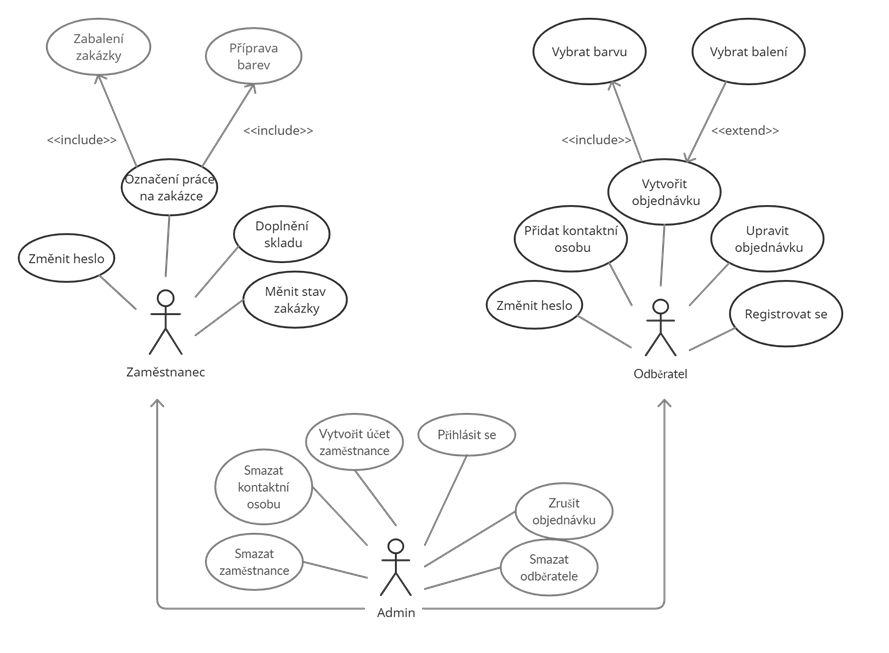
\includegraphics[width=200mm, angle=90]{obrazky-figures/use_case.png}
    \\
    \caption{Diagram případů užití.}
\end{figure}

\newpage



\chapter{Návrh systému}
\label{navrh}

Poté co jsme získali konkrétní požadavky na systém od zákazníka, musíme před implementací nejdříve provést návrh informačního systému. Nejdříve je popsán návrh databáze, který je následně převeden do tabulek relační databáze. Následuje architektonický návrh a návrh uživatelského rozhraní.

\section{ER diagram}
ER diagram(Entity Relationship diagram) je grafický nástroj, který používáme pro návrh databáze. O entitě hovoříme jako o určitém aspektu reálného světa, může to být fyzicky existující objekt jako je například zaměstnanec, výrobek, nebo také událost jako je návštěva lékaře nebo servis automobilu. Součástí každé entitní množiny jsou určité atributy, sloužící k popisu vlastností entitní množiny, například u entity zaměstnanec mohou být atributy: rodné číslo, jméno, příjmení, datum narození a další. Dalším velice důležitým prvkem v ER diagramu jsou vztahy mezi etitními množinami. Vztah se dá chápat jako spojení mezi několika entitami. Spojujeme entity, které spolu logicky souvisí. \cite{erdia} Příklad vztahu může být například žák a třída, protože žák navštěvuje třídu a do třídy chodí několik žáků, proto je potřeba mezi těmito entitními množinami v návrhu vztah znázornit.


\newpage

\begin{figure}[H]
    \centering
    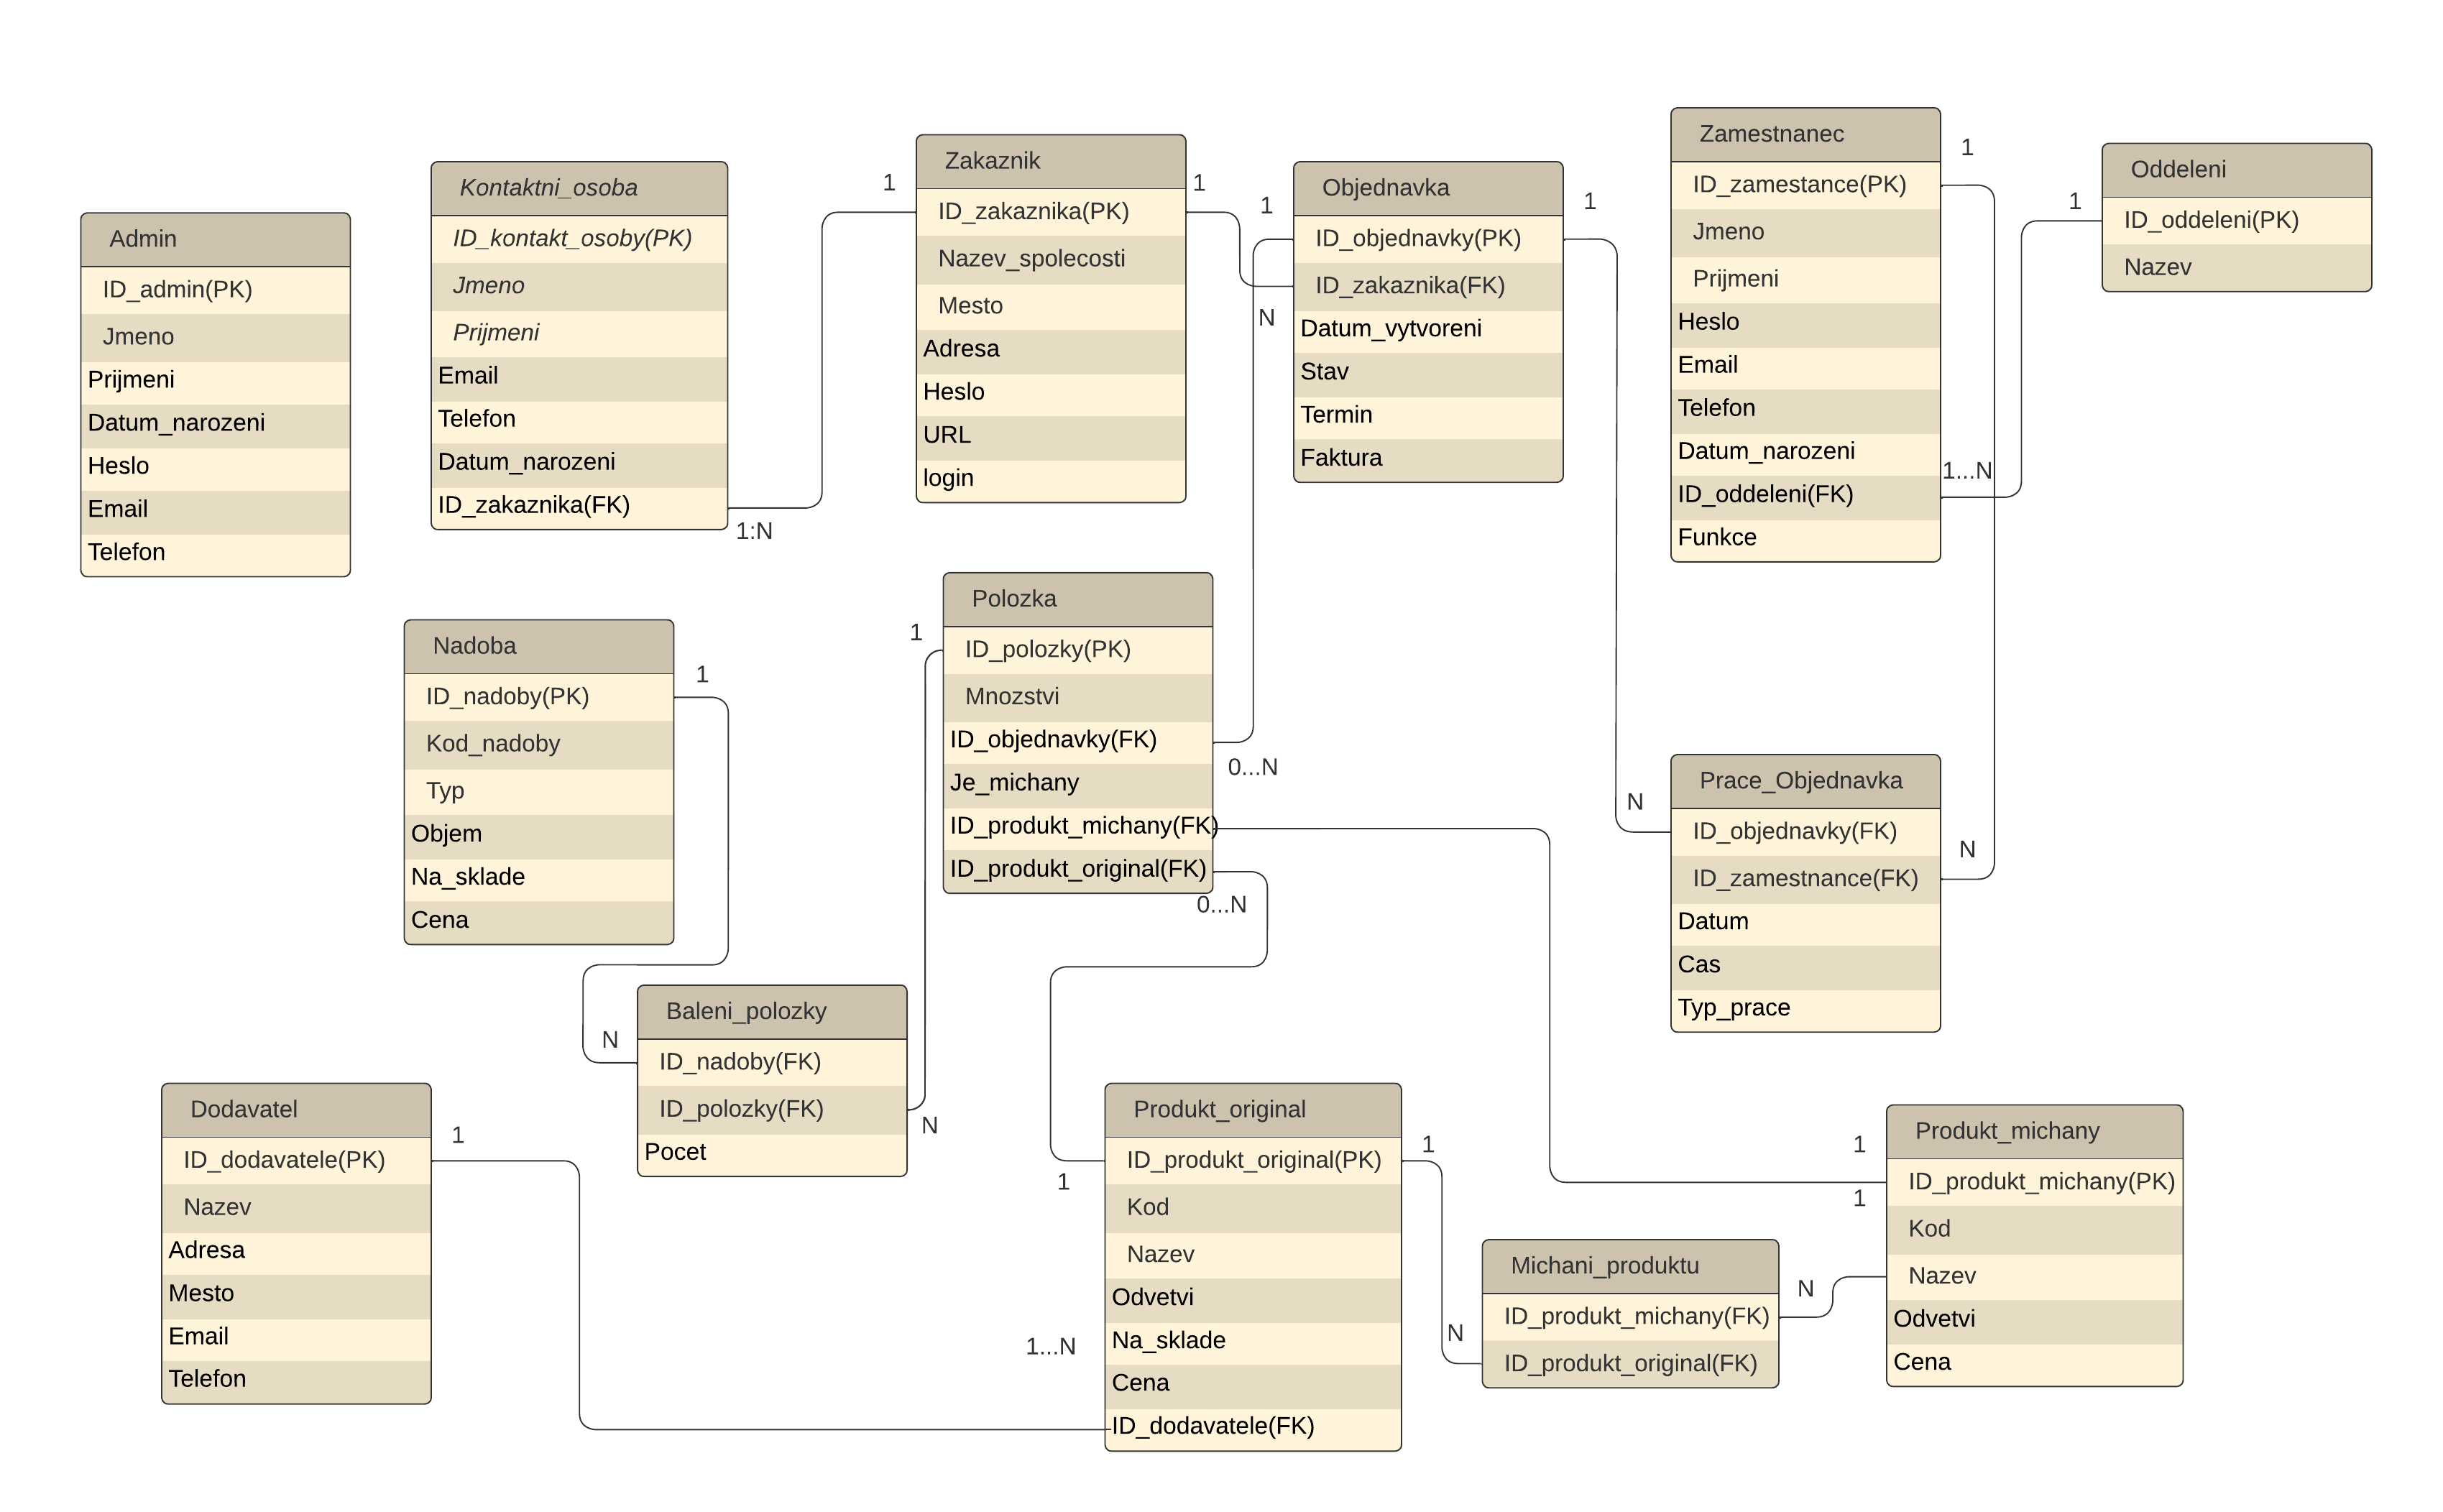
\includegraphics[width=220mm, angle=90]{obrazky-figures/erdiagram.png}
    \\
    \caption{ER diagram.}
\end{figure}

\newpage

\subsection{Admin}
Admin je entitní množina, která ukládá informace o správcích systému. V tabulce admin jsou atributy, které určují kontaktní údaje správce, těmi jsou email nebo telefon, oba tyto atributy musí být unikátní. V tabulce je také atribut \texttt{Heslo}, který se zadává při registraci a pomocí něj a emailu se poté správce do systému přihlašuje.


\subsection{Zákazník}
Entitní množina zákazník nese údaje o všech zákaznících, kteří jsou v systému registrováni a zároveň mají automaticky přidělenou roli zákazníka v systému. V tabulce jsou atributy \texttt{Login} a \texttt{Heslo}, pomocí kterých se zákazník do systému přihlašuje. Dále jsou v tabulce atributy určující polohu firmy(\texttt{Adresa} a \texttt{Mesto}) a také \texttt{URL}, který ukládá url adresu firmy, tento atribut však není povinný.

\subsection{Kontaktní osoba}
Tato entitní množina slouží pro uchovávání kontaktních osob zákazníků. O kontaktních osobách uchováváme informace nutné pro kontaktování osoby, jako jsou email a telefon, dále jméno, příjmení a datum narození. V této entitní množině je cizí klíč odkazující na tabulku \texttt{Zakaznik}, který určuje jakou firmu osoba zastupuje. Každá firma může mít více kontaktních osob. Vztah mezi zákazníkem a kontaktními osobami je 1:N, protože zákazník může mít více kontaktních osob, ale kontaktní osoba zastupuje pouze jednu firmu.


\subsection{Zaměstnanec}
Entitní množina zaměstnanec ukládá údaje o zaměstnancích firmy. Každý zaměstnanec se může přihlásit pomocí emailu a hesla. Dále jsou o zaměstnanci uchovávány v tabulce atributy, sloužící pro jeho kontaktování(\texttt{email} a \texttt{telefon}), datum narození a funkce, který určuje jakou má pracovník  ve firmě funkci. Každý zaměstnanec má v tabulce cizí klíč \texttt{ID\_Oddeleni}, který určuje na kterém oddělení pracuje. 

\subsection{Oddělení}

Entitní množina, která ukládá údaje o odděleních ve firmě. Každý zaměstnanec patří do jednoho oddělení a oddělení má více zaměstnanců, jedná se tedy o vtah 1:N. Tato tabulka má kromě primárního klíče pouze jeden atribut, který určuje název oddělení(\texttt{nazev}).

\subsection{Objednávka}

Entitní množina uchovávající informace o konkrétní objednávce, kterou vytvoří odběratel. Tabulka uchovává atributy data vytvoření objednávky(\texttt{Datum\_vytvoreni}), stav objednávky, ve kterém se právě objednávka nachází(\texttt{stav}) a termín, do kdy je potřeba objednávku připravit(\texttt{termin}).

Entitní množina \texttt{Prace\_objednavka} ukládá údaje o provedené práci na objednávce. Uchovává cizí klíče, které označují zaměstnance(\texttt{ID\_zamestnance}), který práci provedl a na jaké zakázce pracoval(\texttt{ID\_objednavky}). Dále obsahuje atributy určující čas, kdy práci provedl, o jaký typ práce se jedná a také kolik hodin práce trvala.

\subsection{Položka}
Entitní množina \texttt{Polozka} ukládá informace o jednotlivých položkách objednávky. Obsahuje cizí klíč \texttt{ID\_objednavky}, který určuje k jaké objednávce položka patří, dále obsahuje atribut \texttt{mnozstvi}, který určuje množství v litrech. V tabulce je aribut \texttt{je\_michany}, který určuje, zda se jedná o míchaný produkt, který se míchá ve firmě, nebo o originální produkt. Podle toho je konkrétní položka propojena s tabulkou \texttt{Produkt\_original} nebo \texttt{Produkt\_michany}.


\subsection{Nádoba}

Tato entitní množina ukládá údaje o nádobách, ve kterých je možno produkty dodávat. Nese údaje o typu nádoby(\texttt{typ}), tedy jestli se jedná  o kanystr nebo plechovku. Dále obsahuje atributy, které určují jeho cenu, objem a počet kusů na skladě.

\subsection{Balení položky}

Tabulka \texttt{Baleni\_polozky} je propojovací tabulka, která nese informace o tom, jak bude konkrétní položka zabalena. V tabulce jsou cizí klíče \texttt{ID\_nadoby} určující konkrétní nádobu a \texttt{ID\_polozky}, který určuje o jakou položku se jedná. Také je zde atribut \texttt{pocet}, který určuje kolik těchto nádob bude pro položku použito.


\subsection{Originální produkt}

Entitní množina \texttt{Produkt\_original} obsahuje informace o produktech, které jsou dodány do firmy jiným dodavatelem a rovnou jsou přeprodávány zákazníkům bez jakýchkoliv úprav. Každý produkt má svůj unikátní kód, dále jsou ukládány informace o tom, do jakého odvětví produkt patří, cena produktu  a počet litrů na skladě. Dále uchovává cizí klíč určující  výrobce(\texttt{ID\_dodavatele}), který produkt dodal.

\subsection{Dodavatel}

Entitní množina uchovávající údaje o dodavatelích originálních produktů. Obsahuje adresu, kde dodavatel sídlí a také kontaktní údaje jako je email a telefon. Mezi tabulkou \texttt{Dodavatel} a \texttt{Produkt\_original} je vztah 1:N, protože dodavatel může dodávat více originálních produktů, ale produkt může být dodán pouze jedním dodavatelem.

\subsection{Míchaný produkt}

Tato entitní množina reprezentuje produkty, které jsou míchány přímo ve firmě. Nejčastěji se jedná o barvy, které vznikly smícháním originálních produktů. Jako originální produkt tak i každý míchaný má svůj unikátní kód, dále jsou zde uchovány atributy jako je cena za litr nebo odvětví.

\subsection{Míchání produktů}

Entitní množina, která uchovává informace o míchání barev. V tabulce jsou cizí klíče odkazující na originální a míchané barvy.

\section{MVC architektura}

MVC je v dnešní době velice oblíbený architektonický vzor, jehož hlavní myšlenkou je oddělení logiky od výstupu, čímž se aplikace stává znatelně přehlednější. Původně vznikl pro desktop aplikace, ale v dnešní době je využíván zejména pro webové aplikace. Tento model je využíván u mnoha současně oblíbených frameworků jako je již zmíněný Laravel, dále Nette nebo ASP .NET.
Architektura MVC rozděluje aplikace do tří komponent, jimiž jsou: \cite{mvc}


\subsection*{Model}
 Součástí modelu je logika a vše, co se jí týká. Nejčastěji to bývají databázové dotazy nebo výpočty. Funkce modelu spočívá v přijetí vstupních parametrů zvenku a následnému dodání dat ven. Model se nestará o to, odkud data přišla a ani neví v jakém formátu budou výstupní data, tedy vůbec neví o Controlleru a View. \cite{mvc}

\subsection*{View}
View(pohled) zajišťuje zobrazení formátovaných dat uživateli. K zobrazení jsou většinou využívány šablonovací systémy, ve kterých je možno provádět iterace a podmínky. View neví o ostatních komponentách. Neví odkud mu data přišla, pouze je zobrazí uživateli ve správném formátu. \cite{mvc}

\subsection*{Conroller}
Jelikož Model neví o View a naopak, je tedy potřeba zajistit jejich komunikaci. O to se stará právě Controller. Ten komunikuje nejen s View a Modelem, ale také s uživatelem a drží tak celý systém pohromadě. \cite{mvc}

\begin{figure}[H]
    \centering
    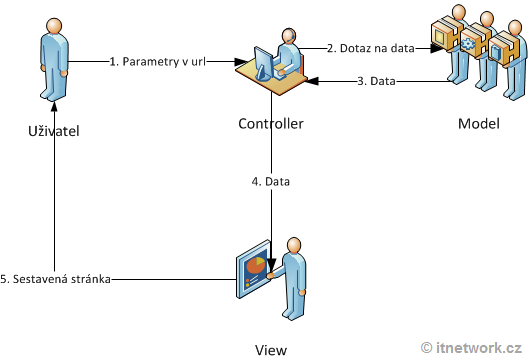
\includegraphics[width=100mm]{obrazky-figures/mvc-itnetwork.png}
    
    \caption{MVC architektura. Převzato z: \cite{mvcimage}.}
\end{figure}


\newpage

\section{Návrh uživatelského rozhraní}

Důležitou součástí informačního systému je uživatelské rozhraní. Při návrhu uživatelského rozhraní je velice důležité, aby bylo přehledné a uživatelsky přívětivé. Je vhodné udělat si hrubý návrh uživatelského rozhraní ještě před implementací, aby jsme se při samotné implementaci nemuseli nesoustředit na to, co vše musíme do uživatelského rozhraní zahrnout.

\subsection*{Návrh stránky s objednávkami}

Pro ukázku jsem si vybral stránku, která bude obsahovat přehled objednávek. Tato stránka je totiž pro uživatele velice důležitá. Součástí informačního systému bude menu, které bude k dispozici ze všech sekcí systému po přihlášené uživatele. Veškeré objednávky budou zobrazeny v tabulce. U každé objednávky budou zobrazeny její vlastnosti jako jsou například: cena, termín, stav a další. Položky se do objednávky budou přidávat po rozkliknutí čísla objednávky.

\begin{figure}[H]
    \centering
    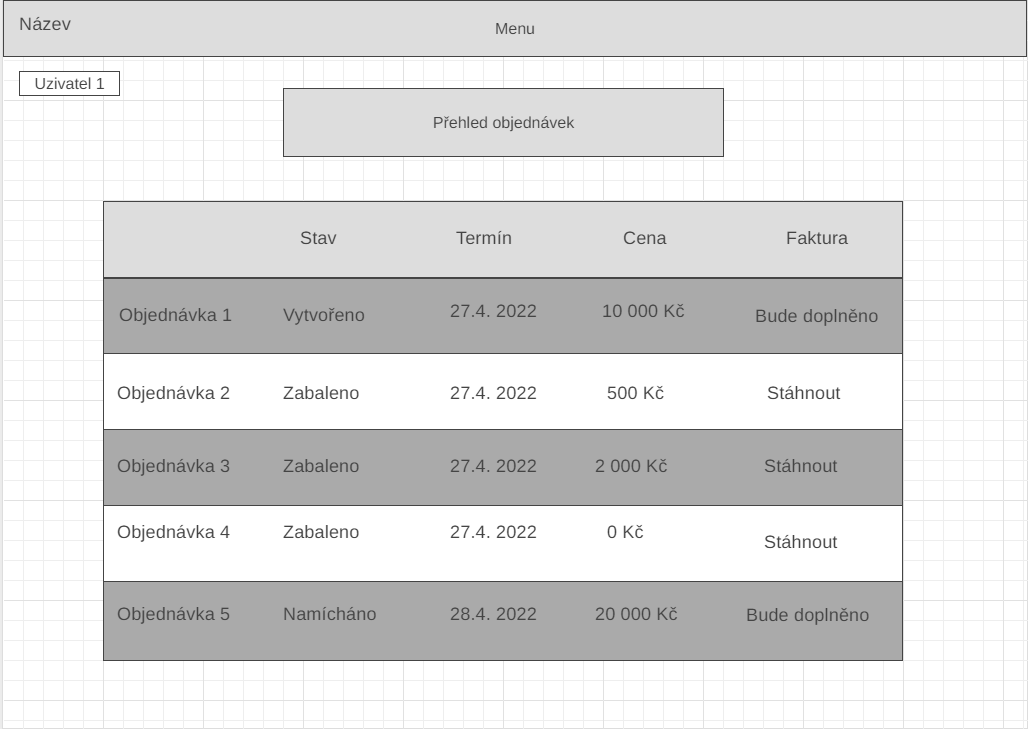
\includegraphics[width=150mm]{obrazky-figures/mockup.png}
    
    \caption{Návrh šablony pro přehled objednávek.}
\end{figure}



\chapter{Použité technologie}
\label{technologies}

V této kapitole jsou rozepsány technologie, které byly použity při tvorbě této práci. Nejdříve je popsán PHP framework Laravel a je porovnán s dalšími frameworky. Poté je popsáno Google Calendar API a na závěr kapitoly jsou popsány front-end technologie.

\section{Back-end technologie}

V této podkapitole se věnuji back-end technologiím, konkrétně PHP frameworkům a jejich vzájemnému porovnání.

\subsection{Laravel}

Laravel\footnote{Dostupné z: \url{https://laravel.com/}.} je PHP framework, který je poskytován zdarma jako open source. V současné době patří k nejpoužívanějším frameworkům. Poprvé byl vydán v roce 2011, vytvořil jej Taylor Otwell a je založen na frameworku Symfony, avšak výhodou je, že není nutná znalost Symfony, k tomu aby  mohl vývojář pracovat s Laravelem. Webové aplikace vytvořené pomocí Laravelu pracují na architektuře model-view-controller(MVC). \cite{laravel} U Laravelu je možnost psát PHP konstrukce přímo do HTML kódu, což nám usnadní mnoho práce a výsledný kód je přehlednější. To umožňuje šablonovací systém blade, který použijeme tak, že za soubor přidáme příponu \texttt{.blade.php}. K instalaci a založení projektu v Laravelu se používá nástroj Composer. Součástí Laravelu je také Artisan.

\subsection*{Composer}

Composer\footnote{Dostupné z: \url{https://getcomposer.org/}.} je nástroj nutný pro založení projektu v Laravelu, protože přes něj probíhá instalace. Composer při instalaci stáhne vše, co je potřeba pro správné fungování Laravelu. Za pomoci composeru můžeme později snadno stahovat a instalovat další knihovny. \cite{composer}

\subsection*{Artisan}

Součástí Laravelu je konzolová aplikace Artisan\footnote{Dostupné z: \url{https://laravel.com/docs/9.x/artisan}.}, která je velmi užitečná a usnadní mnoho práce s vývojem. Artisan se používá pomocí příkazu \texttt{php artisan}, poté se nám zobrazí všechny dostupné příkazy. Pomocí artisanu můžeme vytvářet soubory, jako jsou například Modely nebo Controllery, k vytvoření souboru slouží příkaz: \texttt{php artisan make}. Dále pomocí artisanu probíhají migrace databáze a umožňuje mnoho dalších funkcí, jako například generování registračního a přihlašovacího formuláře. \cite{artisan}




\subsection{Další PHP frameworky}

\subsection*{Symfony}
Dalším frameworkem pro tvorbu webových aplikací v PHP je Symfony\footnote{Dostupné z: \url{https://symfony.com/}.}. Jedná se o open-source framework, který je inspirován například frameworkem Spring nebo Django a sám se stal inspirací pro framework Laravel, který je mu velice podobný. První verze byla vydána v roce 2005 a stále  přicházejí nové inovace, dnes patří k nejpoužívanějším frameworkům na světě. Symfony je stejně jako Laravel postaveno na MVC architektuře. Symfony využívá šablonovací systém Twig, jedná se o obdobu blade u frameworku Laravel. \cite{symfony}


\paragraph{Rozdíly mezi Symfony a Laravelem \cite{laravelsymfony}}
\begin{itemize}
  \item{Laravel je oproti Symfony využíván spíše pro menší projekty, u kterých je důležitá rychlá a jednoduchá implementace a nejsou vyžadovány nestandardní funkce.}
  \item{Symfony je vhodnější pro projekty, u kterých je důležitá dlouhodobá údržba.}
  \item{Laravel má v porovnání se Symfony poměrně snadnou migraci databází a jednoduchou konfiguraci.}
  
\end{itemize}


\subsection*{Nette}
Nette\footnote{Dostupné z: \url{https://nette.org/cs/}.} je, stejně jako Laravel, framework pro tvorbu webových aplikací v PHP. Nette má své kořeny v Česku, původním autorem je David Grudl, z tohoto důvodu je u nás velice rozšířený, ale po světě příliš rozšířený není. Stejně jako Laravel také Nette používá MVC architekturu.


\paragraph{Rozdíly mezi Nette a Laravelem}
\begin{itemize}
  \item{Nette klade větší důraz na bezpečnost výsledné aplikace, obsahuje totiž nástroj, který automaticky generovaný kód ošetřuje od nejčastějších bezpečnostních rizik.}
  \item{Při práci s Nette trvá vývoj webových aplikací delší dobu než u Laravelu.}
  \item{Nette má oproti Laravelu velmi jednoduchou dokumentaci, což je obrovská nevýhoda.}
  
\end{itemize}

\subsection*{CodeIgniter}
Codelgniter\footnote{Dostupné z: \url{https://www.codeigniter.com/}.} je další PHP framework, jehož původní vydání bylo v roce 2006. Codelgniter má výhodu v podobě rychlé přímočaré instalace, u které je vyžadováno jenom minimum konfigurace. Při jeho používání nedochází ke konfliktům kvůli verzím PHP, protože funguje dobře téměř na všech hostovacích platformách.
Oproti Laravelu a mnoho dalších frameworků není striktně založen na MVC architektuře. Je sice nutné používat Controllery, ale modely a pohledy povinné nejsou, můžeme tak používat své vlastní jmenné a kódovací konvence. CodeIgniter tedy vývojářům při vývoji webových aplikací umožňuje značnou volnost, což může být považováno za velkou výhodu. \cite{top10}



\paragraph{Rozdíly mezi Laravelem a CodeIgniterem \cite{codeigniterlaravel}}
\begin{itemize}
  \item{Laravel je relačně objektově orientovaný, zatímco Codeigniter  je pouze objektově orientovaný}
  \item{Laravel přináší funkce ověřování, zatímco CodeIgniter je nepřináší.}
  \item{CodeIgniter oproti Laravelu nepracuje striktně s MVC architekturou.}
  \item{Codeigniter je vhodnější pro začátečníky, protože Laravel nabízí mnoho funkcí, které je složitější pochopit.}
\end{itemize}

\section{Google Calendar}

Google Calendar je internetový kalendář vyvíjen firmou Google od roku 2006. Google Calendar je možné používat prostřednictvím mobilních aplikací na operačních systémech Android i iOS, nebo pomocí webové aplikace. Tento kalendář podporuje spoustu různých funkcí. Události se dají nastavit, tak aby se opakovaly v určitých intervalech, dále si můžeme  nastavovat přesný čas začátku a konce události, nebo nastavit konání na celý den. Je možno natavit místo konání události a také si můžeme nastavit připomenutí pomocí emailu, vyskakovacího okna nebo dokonce bezplatné SMS. Pro vývojářské potřeby je k dispozici vývojové aplikační rozhraní Google Calendar API.

\subsection{Google Calendar API}

Díky Google Calendar API je možné vytvářet aplikace, které mohou pracovat přímo s událostmi v Google kalendáři u zvoleného Google účtu. Google Calendar API je RESTful API, ke kterému můžeme přistupovat prostřednictvím klientských knihoven Google. Toto rozhraní nám zpřístupní většinu funkcí, které jsou dostupné v aplikaci Google Calendar. \cite{calendarapi}

Při práci s Google Calendar API můžeme pracovat s několika komponentami kalendáře, přičemž každá má své vlastní metody, které nám dovolují s nimi pracovat. \cite{calendarapi}

\begin{itemize}
  \item{Event - Event(událost) v kalendáři, jejíž součástí je čas začátku a konce události. Může to být jednorázová událost nebo opakující se událost. }
  \item{Calendar - Kalendář je sbírka akcí. Každý kalendář má svá metadata, která nesou určité vlastnosti, například výchozí časové pásmo kalendáře. }
  \item{Calendar list - Seznam všech kalendářů uživatele v uživatelském rozhraní kalendáře. Metadata obsahují vlastnosti kalendáře specifické pro jednoho uživatele jako je například barva kalendáře nebo způsob upozornění na události.}
  \item{Setting - Předvolby uživatele, například časové pásmo uživatele.}
  \item{ACL - Access control rule(pravidlo řízení přístupu) přiděluje uživateli nebo skupině uživatelů úroveň přístupu ke kalendáři.}
\end{itemize}

\subsection{Příprava pro práci s Google Calendar API}

Ze všeho nejdříve musíme založit nový projekt na domovské stránce Google API. Zadáme název našeho projektu a potvrdíme stisknutím create. Po vytvoření projektu vybereme položku Library, kde jsou API, které si lze aktivovat. My vyhledáme Google Calendar API a aktivujeme. \cite{googleapi}

\begin{figure}[H]
    \centering
    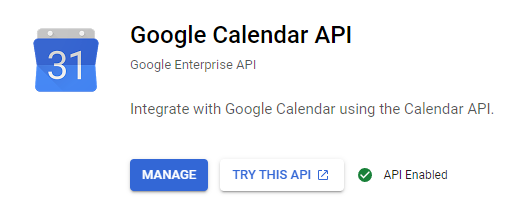
\includegraphics[width=100mm]{obrazky-figures/googlecalapi.png}
    
    \caption{Aktivace Google Calendar API. Převzato z: \cite{googleapi}.}
\end{figure}


Po vytvoření projektu a aktivace Google Calendar API je potřeba vytvořit servisní účet. Účet se vytváří na domovské stránce, musíme vybrat záložku \texttt{Credentials} a poté \texttt{CREATE CREDENTIALS}, otevře se nabídka, ze které vybereme možnost Service Account(servisní účet). Jakmile vytvoříme účet, vygeneruje se nám soubor \texttt{credentials.json}. Díky tomuto souboru můžeme přidávat události do google kalendáře bez autorizace. \cite{cal}


\section{Technologie použité při tvorbě Front-Endu}

Při práci na Front-Endu bylo využito klasické HTML a CSS v kombinaci s frameworkem Bootstrap. Na doplňky ve Front-Endu byl využit jazyk javascript. 

\subsection{Bootstrap} 
Bootstrap\footnote[2]{Dostupné z: \url{https://getbootstrap.com/}.} vytvořil Jacob Thornton a Mark Otto, jedná se o open source framework pro tvorbu webu a webových aplikací, které využívají HTML, CSS a Javascript. Používání bootstrapu je velmi jednoduché, zejména pro vytváření responzivních webů. To je také důvod proč patří mezi nejoblíbenější frameworky současnosti. Při práci lze používat předem definované styly, které lze aplikovat na HTML elementy a není potřeba definovat vlastní styly. Součástí bootstrapu je také používání různých komponent jako jsou například různá tlačítka nebo rozbalovací nabídky a další. \cite{bootstrap}

\subsection{Chart.js} 

Javascriptová knihovna Chart.js\footnote[3]{Dostupné z: \url{https://www.chartjs.org/}.} je open source knihovna, která slouží pro vytváření různých druhů grafů ve webových aplikacích. Chart.js nám umožňuje vymodelovat 8 druhů grafů, pro příklad to jsou grafy: sloupcové, plošné nebo spojnicové. V této práci je tato knihovna využita pro zobrazení statistik prodejních dat. \cite{chart}




\chapter{Implementace}
\label{implementation}

Když máme specifikovány požadavky od zákazníka a máme vytvořen návrh informačního systému, můžeme konečně přistoupit k samotné implementaci. Tato kapitola se věnuje implementaci informačního systému, budou zde popsány různé části informačního systému a postup jejich implementace. Pro implementaci byly využity technologie, které byly popsány v předešlé kapitole.


\section{Důležité soubory}

Jakmile vytvoříme nový projekt v Laravelu, vygeneruje se adresářová struktura s mnoha různými adresáři a soubory. Zde popíšu, se kterými soubory jsem nejvíce pracoval a k čemu slouží.

Nejdůležitějším adresářem je určitě adresář \textbf{app}, obsahuje totiž kódy, které tvoří samotné jádro informačního systému. V něm se nachází podadresář \textbf{Http}, který obsahuje Middlewary a hlavně Controllery, právě Controllery tvoří logiku systému. Dalším podadresářem adresáře \textbf{app} je adresář \textbf{Models}, který obsahuje modely. Každá tabulka v databázi je propojena právě s jedním modelem, který pak nad daty v tabulce provádí změny, jako je přidávání nebo odstraňování záznamů, také provádí dotazy nad tabulkami.

Dalším velmi důležitým adresářem je adresář \textbf{resources}, jehož součástí jsou veškeré pohledy neboli views, tedy soubory, které definují vzhled stránek, které se zobrazují uživateli.

Adresář \textbf{database} obsahuje migrace databáze. Pomocí migrací se vytváří tabulky v databázi.

V kořenovém adresáři je také velice důležitý soubor \textbf{.env}, který obsahuje proměnné prostředí. Můžeme pomocí něj nastavit například přístup k databázi včetně přihlašovacích údajů do databáze.


\section{Připojení a následná práce s databází}

K databázi se připojíme pomocí souboru \textbf{.env} jak již bylo zmíněno dříve. Každá tabulka má svůj vlastní model, těch je v systému okolo patnácti. Abychom mohli později manipulovat s atributy tabulek, musíme je nejdříve do každého modelu zadat.

V modelech se dá snadno definovat vztah mezi tabulkami. Předvedu na příkladu mezi tabulkami \texttt{Zakaznik} a \texttt{Objednavka}, kde je vztah 1:N. Zákazník může mít více objednávek, ale objednávka přísluší pouze jednomu zákazníkovi. V tomto případě vypadá funkce v modelu pro objednávku takto:

\begin{verbatim}
public function customer() { 
    return $this->belongsTo(Customer::class); 
}  
\end{verbatim}


\noindent Funkce v modelu pro zákazníka vypadá pro změnu takto:

\begin{verbatim}
public function order() {
    return $this->hasMany(Order::class);
}
\end{verbatim}



V každém modelu je možné mít funkce, které nějakým způsobem pracují s databází a získávají z nich potřebná data, tyto funkce poté v rámci modelu volají Controllery.


\section{Registrace uživatelů}

Uživatelé se do systému registrují sami, nebo je registruje admin. Registrace je implementována v Controllerech pro registraci. Registrace každé role probíhá ve zvláštním Controlleru.

\subsection{Zákazník}

Pro registraci zákazníka je potřeba vyplnit registrační formulář. Ve formuláři je potřeba vyplnit pole s údaji, některá z nich nejsou povinná. Po vyplnění formuláře a stisknutí tlačítka se zavolá funkce \texttt{store()} v souboru \texttt{CustomerController}. Nejdříve jsou v rámci této funkce data z formuláře zkontrolovány pomocí validátoru. Validátor ověří zda jsou povinná pole opravdu vyplněna, zda jsou ve správném formátu a jsou unikátní v rámci tabulky, pokud je to vyžadováno. Pokud jsou zadané údaje úspěšně validovány, do tabulky zákazníků se vloží záznam s nově vytvořeným zákazníkem. Heslo zákazníka, které se do databáze ukládá je z důvodu bezpečnosti hešováno pomocí funkce \texttt{Hash::make()}. Po vytvoření účtu je zákazník okamžitě přihlášen do systému.

\subsection{Zaměstnanec}

Účet zaměstnance je vytvořen adminem ihned poté, co je do firmy přijat. Admin zaregistruje zaměstnance pomocí registračního formuláře. Další postup je obdobný jako u registrace zákazníka, pouze se zavolá funkce \texttt{store()} ze souboru \texttt{EmployeeController}, data jsou opět nejdříve validována, po úspěšné validaci se vytvoří nový záznam v tabulce zaměstnanců. 

\subsection{Admin}

Admin může přidávat další adminy. Princip vytváření účtu je stejný jako u zaměstnance a zákazníka, pouze se zavolá funkce \texttt{store()} ze souboru \texttt{AdminController}.

\section{Role v systému a jejich autorizace}

Informační systém budou využívat uživatelé tří rolí: admin, zákazník a zaměstnanec. Každému uživateli je přiřazena role podle toho, jakým způsobem se do systému zaregistruje(nebo ho zaregistruje admin). Po vytvoření projektu je v Laravelu pouze jedna role \texttt{user}. Při registraci a přihlašování se automaticky pracuje s tabulkou v databázi \texttt{users}.  Přidání rolí jsem provedl v souboru \texttt{auth.php}, kde jsem nejdříve musel upravit tzv. \textbf{providery}.


\begin{verbatim}
'providers' => [
    'employees' => [
        'driver' => 'eloquent',
        'model' => App\Models\Employee::class,
    ],
],
\end{verbatim}

    
\noindent U každého \textbf{providera} bylo nutné vybrat model, pomocí kterého se po registraci uživatele pozná, jakou roli bude mít. Poté bylo ještě potřeba vytvořit přímo role(tzv. guards):

\begin{verbatim}
'guards' => [
    'employee' => [
        'driver' => 'session',
        'provider' => 'employees',
    ],
],
\end{verbatim}


 U každé z nich jsem vybral providera, kterého jsem již dříve vytvořil. Po této úpravě jsou uživatelům při vytvoření přiřazeny příslušné role. Po vytvoření rolí je nutné nastavit k jakému obsahu webové aplikace budou mít příslušníci každé role přístup. Toto je v informačním systému vyřešeno pomocí tzv. \textbf{Middlewarů}. 
 Zde je příklad využití Middlewaru, v tomto případě se jedná o routu, která provede přesměrování na stránku zobrazení všech zákazníků

\begin{verbatim}
Route::group(['middleware' => 'auth:admin'], function () {
    Route::get('/customers/index',
    [CustomerController::class, 'index'])
    ->name('customers.index');
}
\end{verbatim}



Pokud by cestu této routy zadal příslušník jiné role(v tomto případě zákazník nebo zaměstnanec), byl by ze sytému odhlášen a přesměrován na úvodní přihlašovací obrazovku, kde se může přihlásit jako příslušník jiné role.


\section{Přihlašování do systému}

Přihlašování do systému je provedeno pomocí přihlašovacího formuláře, do kterého zadá uživatel email a heslo, pokud se jedná o admina nebo zaměstnance. V případě, že se však jedná o zákazníka, je nutné, aby zadal login a heslo. Pro přihlášení zákazníků každé role slouží jeden Controller. Pro Zákazníka je to \texttt{LoginCustomerController}, pro admina \texttt{LoginAdminControler} a pro zaměstnance \texttt{LoginEmployeeController}. Každý z těchto Controllerů obsahuje metodu \texttt{index()}, která po zavolání zobrazí uživateli příslušný přihlašovací formulář. V každém tomto Controlleru je také metoda \texttt{login()}, tato metoda slouží k ověření přihlašovacích údajů a následnému přihlášení do systému uživatele s příslušnou rolí. O odhlášení se stará metoda \texttt{logout()}, která je také v každém Controlleru, po odhlášení je uživatel přesměrován zpět na úvodní přihlaovací obrazovku.


\section{Správa uživatelských účtů}

Správu uživatelských účtů si může provést každý uživatel sám různými způsoby. Po vytvoření účtu si zákazník, zaměstnanec i admin mohou upravit svoje údaje, které zadali při registraci. K těmto úpravám slouží stejné Controllery, které sloužili pro registraci uživatelů.  Pokud chce uživatel změnit údaje svého účtu je mu zobrazen formulář pro úpravu profilu pomocí metody \texttt{edit()} v rámci patřičného Controlleru. Ve formuláři jsou již vyplněné jeho původní údaje pro přehlednost, pouze je uživateli stačí přepsat údaji novými. Po vyplnění a kliknutí na tlačítko se zavolá metoda \texttt{update()}, která údaje v databázi změní.

Dále je umožněno uživateli změnit svoje heslo. Uživateli je zobrazen formulář pro změnu hesla, do kterého je nutné zadat staré heslo, nové heslo a zopakovat nové heslo. Heslo je stejně jako při registraci hešováno z důvodu bezpečnosti. 

Úpravu profilu i změnu hesla mohou kromě samotných uživatelů provádět logicky také správci informačního systému. Ti mají možnost zobrazit si seznam všech zaměstnanců a zákazníků. K tomu slouží  \texttt{EmployeeController} a \texttt{CustomerController}, ve kterých je metoda \texttt{index()}, tato metoda vrátí příslušný pohled i s proměnnou, která obsahuje všechny zákazníky nebo zaměstnance, tato proměnná se v pohledu procyklí a do tabulky se vypíšou údaje o patřičných uživatelích. Admin má u každého z těchto uživatelů tlačítko pro změnu hesla i úpravu ostatních údajů.

Správce systému má navíc oproti uživatelům možnost odstranit jejich účty pomocí tlačítka. Po stisknutí tohoto tlačítka je zavolána metoda \texttt{destroy()} s parametrem, který určuje ID uživatele. Tento uživatel je v rámci této metody vyhledán v databázi a jeho účet je odstraněn. U zaměstnanců má navíc admin tlačítko pro označení práce na zakázce. U zákazníka má možnost vytvořit novou objednávku a také přidat novou kontaktní osobu.

\section{Správa produktů v systému}

Produkty se v informačním systému dělí do dvou hlavních skupin, těmi jsou produkty originální a míchané. Originální produkty mají kód produktu začínající písmenem "O" a míchané mají kód začínající písmenem "M". Pro správu produktů slouží soubory \\ \texttt{ProductOriginalController} a \texttt{ProductMixedController}. Produkty může do systému přidávat pouze admin, a to pomocí formuláře. Po zadání potřebných údajů o produktu a kliknutí na tlačítko se zavolá metoda \texttt{store()}, která zařídí uložení produktu do databáze. Produkty může naskladnit zaměstnanec nebo také admin, při zobrazení produktů je u každého z nich textové pole, do kterého se zadá množství, které se naskladní a potvrdí se tlačítkem. Při naskladnění je volána metoda \texttt{addOnStore()}, která změní množství na skladě v databázi. Při naskladnění míchaných produktů se cyklem projdou všechny originální produkty, které jsou v receptu tohoto míchaného produktu a odečtou se ze skladu, protože byly při míchání spotřebovány.

\subsection{Recepty produktů}

Každý míchaný produkt má recept, který obsahuje originální proukty. Vytváření, úprava i odstranění produktu z receptu je prováděna v rámci souboru \texttt{MixingProductController}. Upravit recepty je možno na stránce seznamu produktů, kde je u každého míchaného produktu tlačítko pro změnu receptu. Po stisknutí tlačítka se nám zobrazí pohled \\ \texttt{mixingProduct.show}, kde jsou zobrazeny položky, které jsou již v receptu tohoto produktu. Tuto přísadu je možné smazat.  Dále je zde formulář pro přidání produktu do receptu. Formulář obsahuje pole, do kterého se zadá kód originálního produktu, který chceme do receptu přidat a potvrdí se tlačítkem. Po stisknutí tlačítka se zavolá metoda \texttt{store()}, nejdříve se ověří zda, bylo vyplněno pole originálním produktem, který vážně existuje. Také se ověří, zda tento produkt již není součástí receptu.

\section{Správa objednávek}

Veškerá správa objednávek je prováděna v rámci souboru \texttt{OrderController}. Objednávku může vytvořit zákazník nebo také admin. Zákazník si může vytvořit objednávku při zobrazení svých objednávek, kde stiskne tlačítko pro vytvoření, poté je zavolána metoda \texttt{store()}, která objednávku vytvoří. Admin objednávku vytvoří, když si zobrazí seznam zákazníků a u konkrétního zákazníka stiskne tlačítko pro vytvoření. Poté je zavolána metoda \texttt{storeAdmin()}.

Po vytvoření objednávky mohou k objednávce zaměstnanec nebo admin nahrát fakturu, kterou si později stáhne zákazník. Po nahrání fakturu vidí také admin a zaměstnanec, ti navíc mají možnost fakturu změnit. Při nahrání se zavolá metoda \texttt{uploadFile()}, která soubor uloží do vybraného adresáře a do databáze uloží název tohoto souboru. Pokud je již soubor nahrán, zákazník vidí jeho název a má možnost ho stáhnout.

U každé objednávky je možné po vytvoření měnit její stav(metoda \texttt{changeState()}) a termín(metoda \texttt{changeTerm()}). Termín se zároveň uloží do google kalendáře pomocí Google Calendar API, poté mohou vidět zaměstnanci v google kalendáři termíny objednávek.

\begin{figure}[H]
    \centering
    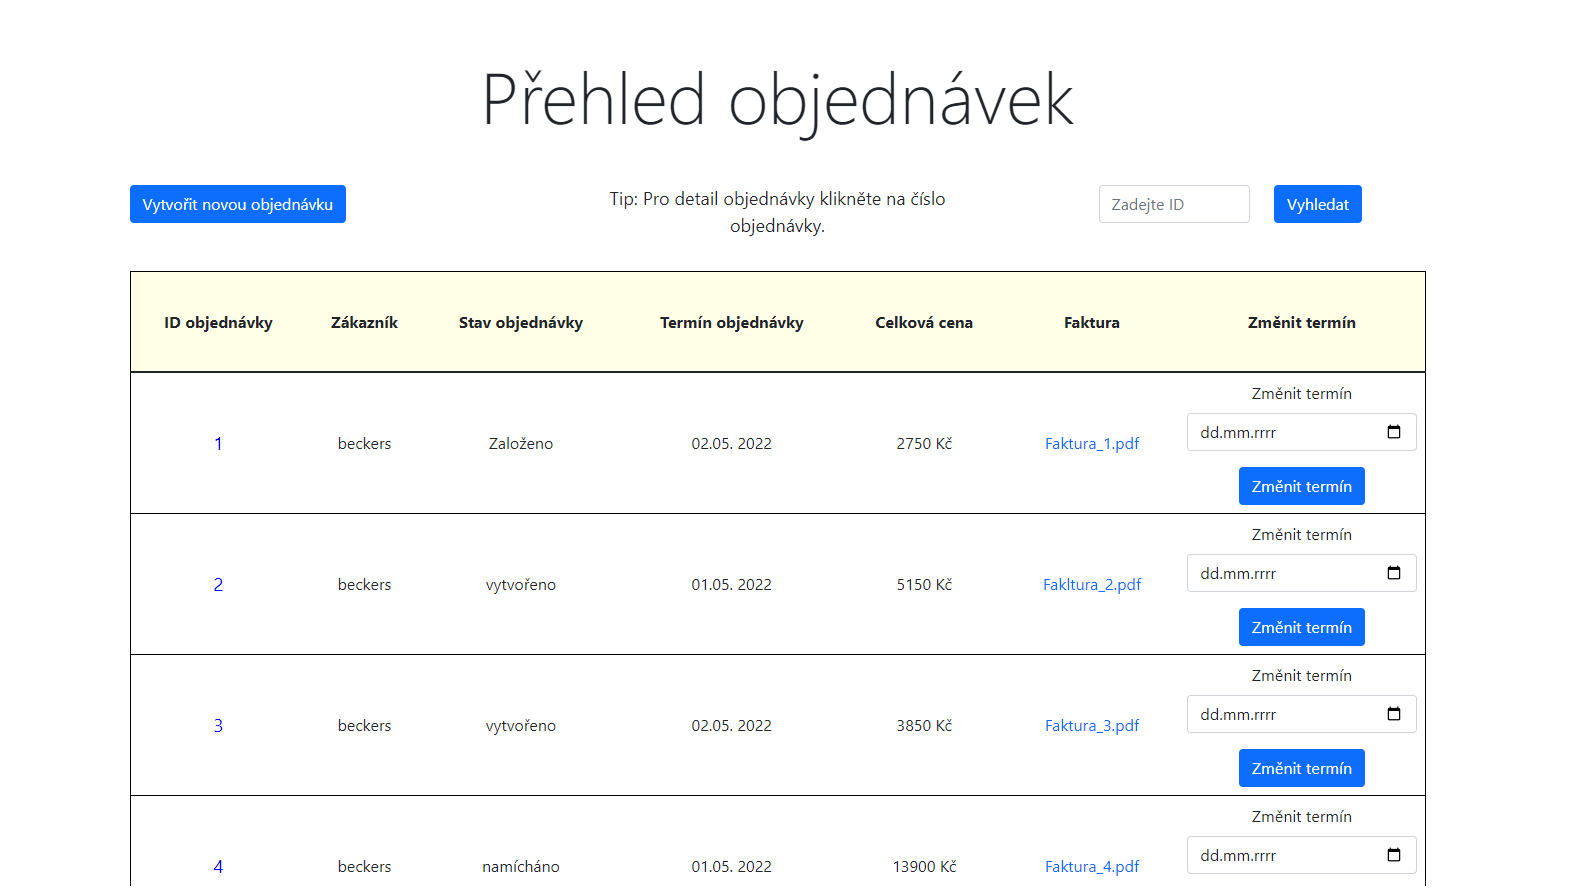
\includegraphics[width=160mm]{obrazky-figures/objednavkyNew.png}
    \caption{Návrh stránky s objednávkami}
\end{figure}




\subsection{Správa položek v objednávce}

S položkami v objednávkách pracuje soubor ItemController. Po rozkliknutí detailu objednávky a kliknutí na tlačítko pro přidání položky se zavolá metoda \texttt{create()}, která zařídí zobrazení seznamu produktů, u kterých bude také textové pole pro zadání množství a tlačítko. Po stisknutí tlačítka se zavolá metoda \texttt{store()}, která nejdříve zjistí podle kódu produktu, zda se jedná o míchaný nebo originální produkt a podle toho vyplní atribut \texttt{is\_mixed} v tabulce s položkami. Také vyplní atribut ID produktu. V rámci této metody se také zkontroluje, zda je na skladě dostatek tohoto produktu, pokud ne, vypíše se varovné hlášení. Pokud je na skladě dostatek kusů, po přidání k objednávce se ze skladu odečtou. Pro odstranění položky z objednávky slouží metoda \texttt{destroy()}, ta naopak po smazání položky automaticky doplní množství na skladě zpět.

\subsection{Správa balení}

Úprava balení položek se provádí v souboru \texttt{PackageItemController}. U každé položky objednávky je tlačítko pro úpravu balení. Po stisknutí vidíme všechny již vybrané nádoby a také tlačítko pro přidání nové nádoby, po stisknutí, stejně jako u produktů, vidíme seznam nádob a textové pole, do kterého zadáme množství kusů. Po přidání je volána metoda \texttt{store()}, která nejdříve zkontroluje počet položek na skladě, v případě, že je na skladě dostatek těchto nádob, přidá do databáze záznam s ID položky, ID nádoby a počtem kusů. Později je možné upravit množství kusů této nádoby, což zařídí metoda(\texttt{changeCount()}) a také je možné nádobu úplně odstranit(metoda \texttt{destroy()}).


\section{Google Calendar}

V informačním systému je využito Google Calendar API, které umožňuje zobrazit přehled objednávek a jejich termíny dokončení v Google kalendáři zaměstnanců. Objednávka je do kalendáře přidána jako celodenní událost na den, kdy je termín této objednávky. Událost je do Google kalendáře přidána při vytvoření objednávky v rámci souboru \texttt{OrderController}. Pro přidávání událostí do kalendáře byla využita tato knihovna: Manage events on a Google Calendar\footnote{Dostupné z: \url{https://github.com/spatie/laravel-google-calendar}}. Ukázka přidání události do google kalendáře je uvedena zde \cite{gitcalendar}: 

\begin{verbatim}
Event::create([
    'id' => 'eventid'.$newOrder->id,
    'name' => 'Číslo objednávky: '.$newOrder->id,
    'startDate' => Carbon::now()->add(1, 'week'),
    'endDate' => Carbon::now()->add(1, 'week'),
]);
\end{verbatim}



Event má několik atributů. Jako identifikátor eventu jsem zvolil řetězec "eventidxx", kde "xx" je ID objednávky, které bude stejné jako v databázi. Počáteční datum události i konečné datum událoti je nastaveno na stejný den, tím se docílí toho, aby byla událost celodenní. V tomto případě je to týden po založení objednávky, protože každá objednávka má po založení tento termín. Při úpravě termínu objednávky se vyhledá událost podle ID objednávky, kterou chceme upravit.

Pokud by událost nebyla nalezena, znamená to, že se z nějakého důvodu při založení objednávky nevytvořila. V tom případě je v rámci tohoto kódu zachycena výjimka \texttt{Google\_Service\_Exception}, poté je tato událost vytvořena znovu. Pokud je událost nalezena, pouze se upraví počáteční a ukončovací datum události.



\section{Asociační pravidla}

V informačním systému je implementováno získávání asociačních pravidel. Konkrétně se vyhledají položky v systému, které jsou často objednávány společně v rámci jedné objednávky a pak je na základě tohoto zjištění zákazníkům doporučováno zboží, které se často vyskytuje s položkami, které již mají v objednávce.

V této práci je využita metoda Apriori. Nalezení frekventovaných množin je řešeno v souboru \texttt{OrderController}, kde je metoda \texttt{getProductsByOrder()}, tato metoda projde celou databázi a vrátí pole, ve kterém jsou na každém indexu uloženy položky, které byly zakoupeny v rámci jedné objednávky. Toto pole je později využito pro získání frekventovaných množin.

Pro implementaci Apriori je využita knihovna PHP-ML\footnote{\url{https://php-ml.readthedocs.io/en/latest/}}. Nejdříve je třeba vytvořit instanci třídy \texttt{Apriori}, do které se zadají parametry podpory a spolehlivosti. Na základě provedeného testování byly zvoleny následující hodnoty, protože při nižší podpoře bylo doporučováno příliš mnoho produktů, při vyšší podpoře naopak byly doporučovány produkty jenom zřídka. 

\begin{verbatim}
$apriori = new Apriori($support = 0.2, $confidence = 0.2); 
\end{verbatim}

 Po vytvoření instance, nad ní zavoláme metodu \texttt{train()}. Jako vstup použijeme pole, které jsme dostali jako výstup funkce \texttt{getProductsByOrder()}. Po vykonání této metody máme vytrénovaný asociátor, můžeme nad ním tedy volat další metody, pomocí kterých získáme potřebné výsledky.

\begin{verbatim}
$apriori->train($items1, $items2);
\end{verbatim}

 Dále bylo vytvořeno pole \texttt{recommendedItems}, do kterého budou uloženy doporučené produkty. Do tohoto pole je uložen výsledek metody \texttt{predict()}, která na vstup dostala pole s produkty, nacházející se v objednávce, pro kterou hledáme doporučené produkty.

\begin{verbatim}
$recommendedItems = $apriori->predict($itemsInOrder);
\end{verbatim}

 Metoda \texttt{predict()} vrátí pole, které obsahuje další pole, ve kterých jsou produkty, které jsou frekventované s produkty v objednávce. Příklad výstupu funkce je uveden zde:

\begin{verbatim}
[[['O-C-4125']], [['M-L-500']], [['O-C-4125', 'M-L-500']]] 
\end{verbatim}

Jelikož se položky v poli vyskytují vícekrát, musely být data upravena tak, aby se každá položka zobrazila uživateli jako doporučené zboží pouze jednou. Tyto data jsou následně odeslána pohledu, který zobrazí detail objednávky. V tomto pohledu jsou poté zobrazeny doporučené produkty pro zákazníka. \cite{apriorilibrary}


\begin{figure}[H]
    \centering
    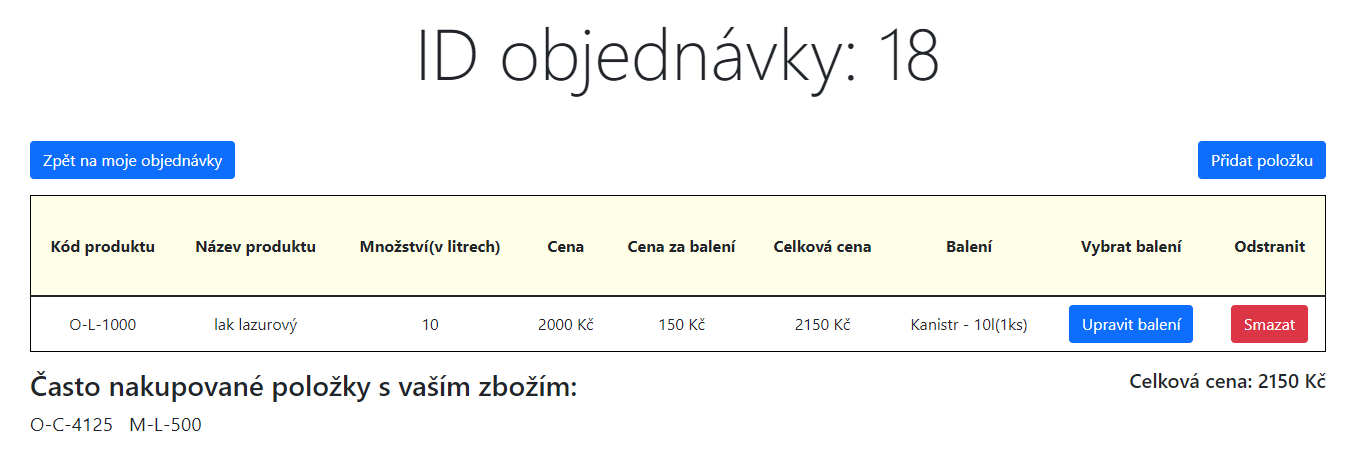
\includegraphics[width=140mm]{obrazky-figures/doporucene.png}
    \caption{Zobrazení doporučených produktů u objednávky}
\end{figure}


\section{Statistiky}
V informačním systému je zpracována analýza dat, která je zobrazena uživatelům systému formou grafů. Uživatelé mají možnost zobrazení statistik týkajících se zejména prodeje produktů, ale také odvedené práce zaměstnanců, nebo největších odběratelů. Ke statistikám mají přístup všichni uživatelé systému, avšak každé roli uživatelů jsou zobrazeny odlišné statistiky. Všechny statistiky vidí pouze admin, zaměstnanec například nevidí statistiky týkající se nejproduktivnějších zaměstnanců a zákazníci nevidí statistiky největších odběratelů.

Pro tvorbu grafů byla využita javascriptová knihovna chart.js\footnote{\url{https://www.chartjs.org/}}. Datová analýza je zpracována v modelu \texttt{Stats.php}, kde jsou volány SQL dotazy nad daty z databáze. Součástí tohoto souboru je také metoda \texttt{getMaxFrom()}, které je jako parametr zadán výsledek dotazu, tato metoda poté vybere záznamy s nejvyšší četností. Metody z tohoto modelu jsou volány v souboru StatsController.php, kde se data z těchto metod uloží do proměnných a jsou odeslány pohledu \texttt{\textbf{stats.\/index.blade.php}}, kde jsou zpracovány formou grafů.

Každý graf je zpracován v jednom canvasu, každý tento canvas má svůj identifikátor, pomocí kterého se určí, který graf do něj bude vymodelován.

Zde vidíme příklad dotazu, jehož výsledkem je seznam zaměstnanců a součet hodin, které odpracovaly.


Na obrázku \ref{fíg:img1} vidíme nejprodávanější produkty vymodelované do sloupcového grafu. Na  obrázku \ref{fig:img2} vidíme podíl nádob, ve kterých jsou produkty doručovány.  Data jsou vymodelována do koláčového grafu, ve kterém jsou uvedeny procenta, které nám říkají v kolika případech jsou produkty doručovány v plechovkách a v kolika případech v kanystrech.

\begin{figure}[H]
\begin{center}
    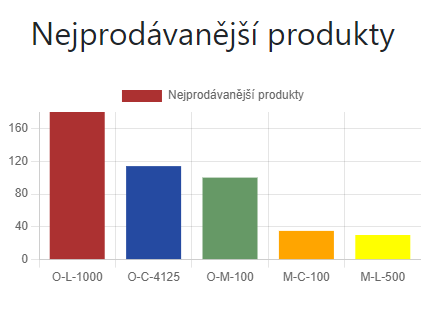
\includegraphics[width=80mm]{obrazky-figures/stat.png}
    
    \label{fíg:img1}
    \caption{Ukázka sloupcového grafu grafu}
\end{center}
\end{figure}



\begin{figure}[H]
    \begin{center}
    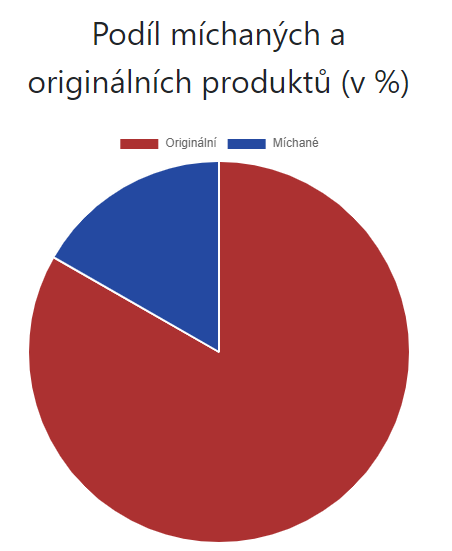
\includegraphics[width=70mm]{obrazky-figures/stat2.png}
    
    \label{fig:img2}
    \caption{Ukázka koláčového grafu}
\end{center}
\end{figure}


\newpage

\chapter{Testování}
\label{test}

Posledním krokem, který následoval po implementaci bylo testování výsledné aplikace. Jedná se o velice důležitou fázi, při které ověřujeme, zda funguje výsledný produkt tak, jak se očekává.

\section{Testování při implementaci}

Po implementaci každé větší části informačního systému bylo provedeno testování. Při tomto testování byly odhaleny drobné chyby, které se týkaly například chybného předávání parametrů mezi třídami a šablonami. Také často bylo zapotřebí opravit chybové hlášky. Toto testování probíhalo na lokálním serveru a aplikace pracovala s lokální MySQL databází.

\section{Testování uživateli}

Jakmile byla implementace informačního systému dokončena začalo uživatelské testování. Při tomto testování bylo hlavním účelem zjistit výslednou kvalitu systému v praxi. Také bylo potřeba ověřit, zda jsou správně splněny všechny požadavky na výsledný systém. Tohoto testování se účastnila firma, která je potencionálním zákazníkem. Dále systém testovaly příslušníci rodiny, přátelé a blízcí.

\subsection*{Kroky, které provedly zákazníci}

Nejdříve ze všeho zákazník dostal za úkol vytvořit si svůj účet v systému a následně se přihlásit. Po přihlášení si vyzkoušel změnit svoje heslo a také některé údaje, které zadal při registraci. Poté si v systému prohlédl nabízené produkty a vytvořil si novou objednávku, do objednávky si přidal několik produktů a vybral jejich zabalení. Do několika objednávek zákazník přidal stejné produkty a vyzkoušel jestli v další objednávce dostane doporučení na produkty, které se opakují v již vytvořených objednávkách. U objednávky si poté stáhnul fakturu a také si zkusil změnit termín, do kterého chce mít objednávku připravenou. Po otestování objednávek si zkusil přidat novou kontaktní osobu, změnit její údaje a následně ji zkusil také smazat. Jako poslední krok bylo odhlášení ze systému.

\subsection*{Kroky, které provedly zaměstnanci}

Zaměstnanec dostal přihlašovací údaje, pomocí kterých se do systému přihlásil. Po přihlášení změnil svoje údaje a heslo. Poté změnil stav objednávek a označil na objednávkách vykonanou práci, svoji odvedenou práci si zobrazil a zkontroloval. K objednávce nahrál fakturu. V rámci svého Google účtu si zkusil do svého Google kalendáře přidat firemní kalendář, ve kterém se mu zobrazují termíny všech objednávek. Po splnění těchto úkolů se odhlásil ze systému.


\chapter{Závěr}
\label{end}

Cílem této bakalářské práce bylo navrhnout a implementovat informační systém pro prodejce nátěrových hmot. Při návrhu i implementaci byl kladen důraz zejména na přehlednost a jednoduchost systému. Při vývoji informačního systému byly pořádány konzultace s potencionálním zákazníkem, tak aby výsledný systém co nejvíce odpovídal jeho požadavkům. V rámci systému je zákazníkům umožněno prohlížet si dostupné produkty, vytvářet nové objednávky, do kterých přidávají produkty a vybírají si u nich konkrétní zabalení. U každé objednávky si zákazník může nastavit termín, do kterého chce mít objednávku vyřízenou. Zaměstnanec má přehled o všech objednávkách, může měnit jejich stav a označovat na nich vykonanou práci. Pro lepší přehlednost o termínech objednávek je zaměstnancům umožněno propojení s Google kalendářem, ve kterém se všechny termíny zobrazí. Kromě těchto bodů, je poskytnuto zobrazení statistik týkajících se prodeje produktů a dalších dat v systému. Také je implementována analýza sociačních pravidel, pomocí kterých jsou zákazníkům doporučovány produkty v závislosti na produktech, které jsou součástí objednávky. Informační systém je dostupný online na webové adrese: \url{http://bakal-colors.online/}.

\section{Možná vylepšení}

Informační systém vyhovuje všem požadavkům, které zákazník požadoval, avšak jsou určitá vylepšení, která by mohla být do budoucna implementována. Jedno z těchto vylepšení by mohla být pokročilejší analýza pomocí OLAP technologií, například by mohly být dostupné statistiky, které by ukazovaly nejprodávanější produkty v závislosti na ročních obdobích. Také by mohlo být implementováno využití nějaké shlukovací metody, například pro shlukování zákazníků, kteří často nakupují stejné produkty. Systém by do budoucna mohl navíc obsahovat volbu dopravy. Kromě webové aplikace by systém mohl být také součástí mobilní aplikace, aby zákazník mohl snáze vytvářet a spravovat své objednávky.




